% Active Foveal 3-D Vision -- technical report (REVIEW DRAFT).
% Build: see README.md in this directory (pdflatex -> bibtex -> pdflatex x2; no experiment is required).
\documentclass[11pt,a4paper]{article}

\usepackage[T1]{fontenc}
\usepackage[utf8]{inputenc}
\usepackage{lmodern}
\usepackage[a4paper,top=2.5cm,bottom=2.6cm,left=2.6cm,right=2.6cm,headheight=14pt]{geometry}
\usepackage{microtype}
\usepackage{amsmath,amssymb}
\usepackage{graphicx}
\usepackage{booktabs}
\usepackage{tabularx}
\usepackage{array}
\usepackage{xcolor}
\usepackage{enumitem}
\usepackage[font=small,labelfont=bf,margin=0pt]{caption}
\usepackage{subcaption}
\usepackage{tikz}
\usetikzlibrary{arrows.meta,positioning,calc,fit,backgrounds}
\usepackage{pgfplots}
\pgfplotsset{compat=1.18}
\usepackage[round]{natbib}
\usepackage{fancyhdr}
\usepackage[hidelinks]{hyperref}
\hypersetup{colorlinks=true,linkcolor=black!70!blue,citecolor=black!70!blue,urlcolor=black!70!blue,
  pdftitle={Active Foveal 3-D Vision},pdfauthor={Luiz Velho}}

% ---------------------------------------------------------------- Visual Language 1 colours (Okabe-Ito based)
\definecolor{oiblue}{RGB}{0,114,178}
\definecolor{oisky}{RGB}{86,180,233}
\definecolor{oiverm}{RGB}{213,94,0}
\definecolor{oiorange}{RGB}{230,159,0}
\definecolor{oigreen}{RGB}{0,158,115}
\definecolor{depthblue}{RGB}{0,92,150}
\definecolor{seenblue}{RGB}{166,196,222}
\definecolor{unseengrey}{RGB}{236,235,230}
\definecolor{coveredgreen}{RGB}{178,214,196}
\definecolor{inkc}{RGB}{38,38,38}
\definecolor{bA}{RGB}{198,219,239}\definecolor{bB}{RGB}{158,202,225}\definecolor{bC}{RGB}{107,174,214}
\definecolor{bD}{RGB}{66,146,198}\definecolor{bE}{RGB}{33,113,181}\definecolor{bF}{RGB}{8,81,156}
\definecolor{bG}{RGB}{8,48,107}
\pgfdeclarehorizontalshading{depthramp}{100bp}{color(0bp)=(bA); color(16.7bp)=(bB); color(33.3bp)=(bC);
  color(50bp)=(bD); color(66.7bp)=(bE); color(83.3bp)=(bF); color(100bp)=(bG)}

% ---------------------------------------------------------------- small helpers
\newcommand{\truth}[1]{{\sffamily\footnotesize\textbf{#1}}}
\newcommand{\code}[1]{\texttt{\small #1}}
\newcommand{\Hz}{\ensuremath{\mathrm{H}_0}}
\newcommand{\pct}[1]{#1\,\%}
\newcommand{\degr}{\ensuremath{^\circ}}
\newcommand{\depthbar}[1]{% #1 = width
  \begin{tikzpicture}[font=\sffamily\scriptsize]
    \shade[shading=depthramp] (0,0) rectangle (#1,0.18);
    \draw[black!40] (0,0) rectangle (#1,0.18);
    \foreach \m in {1,2,3,4,5} {\pgfmathsetmacro{\x}{(\m-0.5)/5*#1}
      \draw[black!55] (\x,0) -- (\x,-0.06) node[below, inner sep=1pt] {\m\,m};}
  \end{tikzpicture}}

\setlist{itemsep=2pt,topsep=4pt,parsep=0pt}
\setlength{\parskip}{3pt}
\renewcommand{\arraystretch}{1.12}

\pagestyle{fancy}
\fancyhf{}
\fancyhead[L]{\small\sffamily Active Foveal 3-D Vision}
\fancyhead[R]{\small\sffamily Technical report --- review draft}
\fancyfoot[C]{\small\thepage}
\renewcommand{\headrulewidth}{0.3pt}

\begin{document}

% ================================================================ title block
\thispagestyle{plain}
\begin{center}
  {\fontsize{24}{28}\selectfont\bfseries Active Foveal 3-D Vision}\\[8pt]
  {\large A Fixate--Reconstruct--Saccade Playground\\ for 360-Degree Scene Reconstruction}\\[9pt]
  {\itshape A controlled proof of concept and reproducible computational baseline}\\[16pt]
  {\large Luiz Velho}\\[2pt]
  VISGRAF Laboratory, IMPA\\[7pt]
  {\footnotesize Developed in collaboration with\\
  ChatGPT --- GPT-5.6 Sol, OpenAI\\
  Claude Code --- Claude Opus 5.5, Anthropic}\\[9pt]
  October 2026\\[5pt]
  {\footnotesize\sffamily\bfseries TECHNICAL REPORT --- REVIEW DRAFT}
\end{center}
\vspace{4pt}

\begin{abstract}
\noindent
Biological vision does not capture the world at full resolution all at once. A small, high-acuity fovea is moved by
saccades, and a persistent percept is assembled over time. We study the computational counterpart of this
observation: can a spatially selective binocular observer, with a fixed head, build a persistent metric 3-D
representation of its whole surroundings by deciding where to look? We describe a deliberately small architecture
built around one loop---fixate, reconstruct everything the fovea can measure, update a global memory, saccade---and a
reproducible implementation of it, the Greedy Foveal Explorer. Each fixation measures a 12\degr{} binocular foveal
core. Correspondence is supplied by a PERFECT / ORACLE service derived from the renderer, and metric points come from
spherical epipolar triangulation into a fixed head frame. A persistent surfel map accumulates the geometry, and a
1\degr{} cyclopean sphere records which directions have been seen. Gaze selection uses only that sphere and the current
fixation's evidence, not the accumulated map. In a static synthetic Blender Classroom, the explorer stopped itself
after 542 fixations (322 local and 219 global saccades), with \pct{99.00} of the sphere seen and \pct{98.28} with
reconstructed depth. Its 16{,}517{,}811-surfel map reconstructs \pct{98.32} of the first-hit reference solid angle
within 12\,mm; the reference was opened only after the run was frozen. An official reproduction is bitwise identical
to the frozen baseline in every control-path product. We present the system as a controlled proof of concept and as
an experimental playground, in which individual components can be replaced one at a time and compared against this
baseline.
\end{abstract}

% ================================================================ 1
\section{Introduction}

A conventional camera tries to capture an entire field of view at uniform resolution in a single exposure. Animal
vision works differently. Only a small central region of the retina resolves fine detail, and the eyes move several
times per second to bring different parts of the scene onto it. What we experience as a stable, detailed, wide visual
world is assembled over many brief fixations \citep{yarbus1967}. This report asks whether that strategy can be turned
into a working computational baseline for 3-D perception.

The question is therefore not
\begin{quote}
\itshape How can a camera capture everything at maximal resolution at once?
\end{quote}
but rather
\begin{quote}
\itshape Can a spatially selective binocular observer build a persistent 3-D representation by deciding where to look?
\end{quote}
The answer we pursue is an additive one:
\begin{center}
local high-quality measurement \;$+$\; eye movements \;$+$\; persistent memory\\[2pt]
$=$\; virtual wide-field perception over time.
\end{center}
A narrow fovea that is moved deliberately, and whose measurements are remembered in a common frame, behaves over time
like a wide-field sensor, even though at no single moment does it see more than 12\degr{} of the world in detail.

We built the smallest architecture we could find that makes this concrete. A fixed binocular head sits in a static
scene. At each step it fixates, reconstructs everything the fovea can match into metric 3-D, adds the result to one
persistent map and to a coarse record of where it has looked, and chooses its next gaze with a simple greedy rule.
Stereo correspondence is supplied by a PERFECT / ORACLE service derived from the renderer. This assumption is
deliberate: it separates the questions of \emph{exploration} and \emph{accumulation}, which this report addresses, from
the question of \emph{natural stereo matching}, which it does not.

\paragraph{Contribution.} The contribution is modest and, we hope, useful:
\begin{enumerate}
  \item a clean active-foveal architecture with explicit persistent state and separable services
        (Sections~\ref{sec:playground}--\ref{sec:policy});
  \item a demonstration that, in a controlled synthetic setting, a very simple greedy gaze policy suffices to observe
        \pct{99} of the sphere and to reconstruct nearly the whole first-hit 360\degr{} scene metrically
        (Sections~\ref{sec:classroom}--\ref{sec:results});
  \item a reproducible computational baseline---official code, frozen run, bitwise reproduction and a truth firewall
        between control and evaluation---organized as a playground in which one component at a time can be replaced
        and measured (Sections~\ref{sec:software} and~\ref{sec:extension}).
\end{enumerate}
We do not claim optimal gaze control, natural stereo, natural segmentation, or generalization beyond the scene studied
here.

\paragraph{How claims are labelled.} Numbers in this report are of four kinds. \truth{MEASURED} values come from an
identified run; unless stated otherwise, the official reproduction of Section~\ref{sec:equivalence}.
\truth{PARAMETER} values are configured settings. \truth{DERIVED} quantities and images are computed from run products.
\truth{REFERENCE / EVALUATION} denotes the independent Blender reference used only after a run is frozen. Information
that comes from the renderer's internal geometry is called \truth{ORACLE} and is used only where declared: for
correspondence, and for visualization.

\paragraph{Outline.} Section~\ref{sec:background} places the work in the active-vision tradition.
Sections~\ref{sec:playground}--\ref{sec:policy} describe the architecture: the loop and its state, the geometry, a
single fixation, the persistent map, the coverage memory and the gaze policy. Section~\ref{sec:software} covers the
implementation and its reproducibility. Sections~\ref{sec:classroom} and~\ref{sec:results} present the Classroom
experiment and its results, Section~\ref{sec:discussion} discusses them, Section~\ref{sec:extension} lays out the
playground, and Sections~\ref{sec:limitations} and~\ref{sec:conclusion} close.

% ================================================================ 2
\section{Background and design motivation}\label{sec:background}

\paragraph{Fixation, saccades and persistent perception.} Yarbus's recordings of eye movements during picture viewing
showed that gaze does not sweep a scene uniformly. It dwells on informative regions, in patterns that depend on the
scene and on the observer's task, and perception is built across a sequence of fixations
\citep{yarbus1967}. Three ingredients of that picture shape the present design: a small region of high-quality
sensing, discrete gaze shifts between fixations, and a percept that persists across them.

\paragraph{Active vision.} \citet{aloimonos1988} argued that an observer that controls its own sensor geometry can turn
problems that are ill-posed or unstable for a passive observer into well-posed and stable ones. Sensing becomes part of
a loop with action. Our explorer is active in exactly this sense: each measurement exists because the system chose to
make it, and what it measures depends on where it chose to look.

\paragraph{Animate vision.} \citet{ballard1991} argued that a system able to control its gaze can exploit fixation, and
the coordinate frames it induces, to simplify visual computation, instead of reconstructing everything from a passive
image stream. We adopt this computational stance. The local measurement is defined relative to the current fixation (a
gaze-centred tangent frame and the eye pair's epipolar geometry), and only its result is moved into a common,
persistent frame.

\paragraph{Space-variant sensing.} \citet{schwartz1995} reviewed space-variant active vision, in which a sensor trades
uniform resolution for a high-resolution centre and a coarse periphery. That trade only makes sense with active gaze
control, because the sensor must be pointed at whatever needs detail. The underlying principle---high resolution does
not need to exist everywhere at once---is the premise of this project.

\paragraph{What this baseline uses.} The present implementation does \emph{not} model a variable-resolution retina. Each
eye renders a uniform perspective image, and the central 12\degr{} of it serves as a nominal foveal core; peripheral
pixels are not used. Variable-resolution retinal sampling belongs to the larger vision of the project, but this
baseline does not need it. Its questions are about exploration and accumulation: given a narrow, high-quality
binocular measurement, where should it be pointed, and how should the results be remembered?

% ================================================================ 3
\section{The active foveal playground}\label{sec:playground}

\paragraph{Design principle.} The whole system is one loop:
\begin{center}
\sffamily FIXATE $\;\rightarrow\;$ RECONSTRUCT EVERYTHING LOCALLY $\;\rightarrow\;$
UPDATE GLOBAL \Hz{} MAP + CYCLOPEAN COVERAGE $\;\rightarrow\;$ LOCAL OR GLOBAL SACCADE $\;\rightarrow\;$ REPEAT
\end{center}
Each fixation is self-contained. The observer points both eyes at a gaze direction, measures every foveal pixel it can
match between the two eyes, and expresses the result in a fixed head frame \Hz{}. It fuses the result into one global
map and records the observed directions on a coarse sphere. A simple rule then chooses the next gaze: a short step to a
neighbouring view when the fovea's own measurement shows surface continuing in an unexplored direction, or a jump to
the middle of the largest unexplored region otherwise. The loop stops when \pct{99} of the sphere has been seen.

\paragraph{Persistent state.} Only four things persist from one fixation to the next (Table~\ref{tab:state}). Nothing
object-centric is needed: there are no object hypotheses, no object list, no per-object maps and no scheduler.

\begin{table}[h]
\centering\small
\caption{Persistent state of the baseline. Everything else is rebuilt at every fixation and discarded. The last
column is the key architectural fact: the gaze policy does not read the map.}
\label{tab:state}
\begin{tabularx}{\linewidth}{@{}l X l c@{}}
\toprule
& state & updated by & read by gaze policy \\
\midrule
$M$ & global \Hz{} surfel map: position (float64, metres), blended RGB, support count, first fixation, oracle label
      (visualization only) & 12-mm fusion, every fixation & \textbf{no} \\
$S$ & cyclopean sphere: $180\times360$ cells of 1\degr{}, each \textsc{unseen}, \textsc{seen} or \textsc{depth} &
      coverage update, every fixation & yes \\
$V$ & visited gaze directions (unit vectors in \Hz{}) & appended every fixation & yes \\
$g$ & current gaze (yaw, pitch) in \Hz{} & the saccade decision & yes \\
\midrule
--- & \emph{transient:} valid-geometry mask of the current foveal core & reconstruction & yes (then discarded) \\
\bottomrule
\end{tabularx}
\end{table}

Figure~\ref{fig:loop} shows the loop and its data flow. It distinguishes the observation, the derived metric
reconstruction, the persistent memory and the action. The global map $M$ is the principal geometric output of the
system, and it is \emph{not} an input to gaze selection. The policy reads the coverage sphere $S$, the visited
directions $V$ and the current fixation's valid-geometry evidence. This is intentional. It keeps the baseline minimal,
and it leaves open one of the most interesting playground questions: what changes when attention is driven by the
reconstructed 3-D map itself (Section~\ref{sec:discussion})?

\begin{figure}[t]
\centering
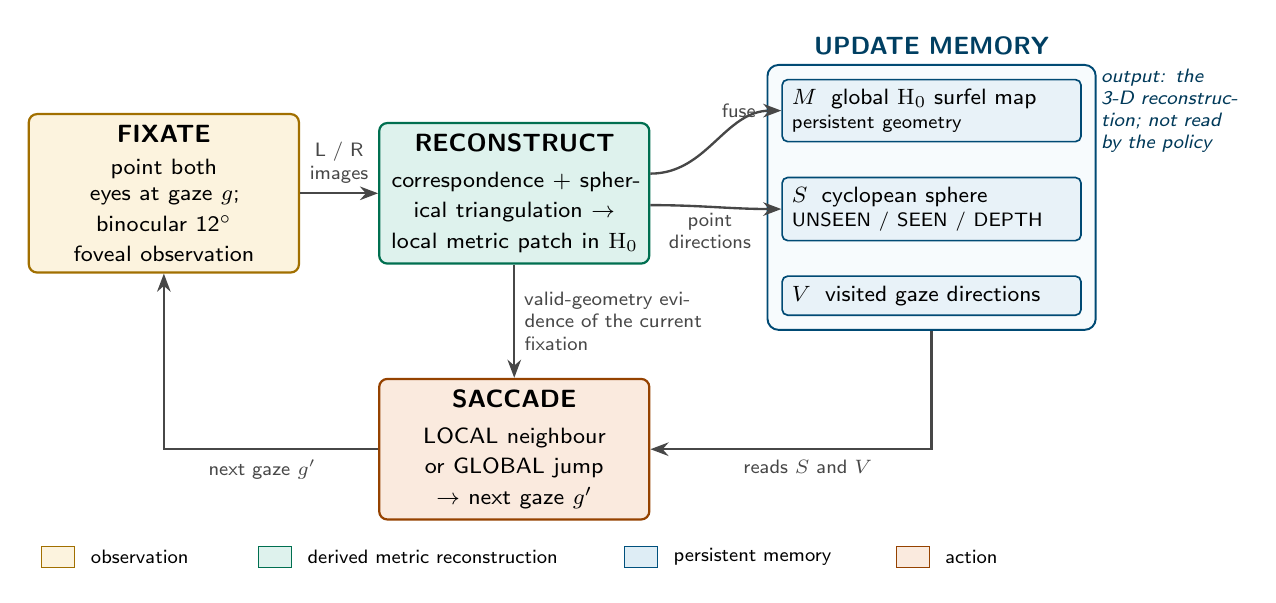
\begin{tikzpicture}[
  font=\sffamily\small, >={Stealth[length=2.3mm]},
  stage/.style={rounded corners=3pt, draw=#1!70!black, fill=#1!13, line width=0.8pt, align=center,
                minimum height=1.6cm, text width=3.15cm, inner sep=4pt},
  mem/.style={rounded corners=2pt, draw=oiblue!65!black, fill=oiblue!9, line width=0.6pt, align=left,
              text width=3.55cm, inner sep=3.5pt, font=\sffamily\footnotesize},
  lab/.style={font=\sffamily\scriptsize, text=black!72, align=center},
  flow/.style={->, line width=0.85pt, black!72},
]
\node[stage=oiorange] (fix) at (0,0) {\textbf{FIXATE}\\[2pt]\footnotesize point both eyes at gaze $g$;\\
  binocular 12\degr{} foveal observation};
\node[stage=oigreen] (rec) at (4.45,0) {\textbf{RECONSTRUCT}\\[2pt]\footnotesize correspondence + spherical
  triangulation $\rightarrow$ local metric patch in \Hz{}};
\node[mem] (M) at (9.75,1.05) {\textbf{$M$}\; global \Hz{} surfel map\\[-1pt]{\scriptsize persistent geometry}};
\node[mem] (S) at (9.75,-0.2) {\textbf{$S$}\; cyclopean sphere\\[-1pt]{\scriptsize UNSEEN / SEEN / DEPTH}};
\node[mem] (V) at (9.75,-1.3) {\textbf{$V$}\; visited gaze directions};
\begin{scope}[on background layer]
\node[draw=oiblue!65!black, fill=oiblue!3, rounded corners=4pt, fit=(M)(S)(V), inner sep=5pt, line width=0.7pt]
  (memblock) {};
\end{scope}
\node[font=\sffamily\small\bfseries, text=oiblue!55!black, anchor=south] at (memblock.north) {UPDATE MEMORY};
\node[stage=oiverm] (sac) at (4.45,-3.25) {\textbf{SACCADE}\\[2pt]\footnotesize LOCAL neighbour or GLOBAL jump
  $\rightarrow$ next gaze $g'$};
\draw[flow] (fix) -- node[above, lab]{L / R\\images} (rec);
\draw[flow] ($(rec.east)+(0,0.25)$) to[out=0, in=180] node[above, lab, pos=0.7, inner sep=2pt]{fuse} (M.west);
\draw[flow] ($(rec.east)+(0,-0.15)$) to[out=0, in=180] node[below, lab, pos=0.45, inner sep=2pt]{point\\directions} (S.west);
\draw[flow] (rec.south) -- node[right, lab, text width=2.3cm, align=left]{valid-geometry evidence of the current
  fixation} (sac.north);
\draw[flow] (memblock.south) |- node[pos=0.72, below, lab]{reads $S$ and $V$} (sac.east);
\draw[flow] (sac.west) -| node[pos=0.27, below, lab]{next gaze $g'$} (fix.south);
\node[lab, anchor=west, text width=1.75cm, align=left, text=oiblue!50!black] at ($(M.east)+(0.12,0)$)
  {\textit{output: the 3-D reconstruction; not read by the policy}};
% legend
\begin{scope}[shift={(-1.55,-4.75)}, font=\sffamily\scriptsize]
  \foreach \c/\t/\xx in {oiorange/observation/0, oigreen/derived metric reconstruction/2.75,
                          oiblue/persistent memory/7.4, oiverm/action/10.85} {
    \fill[\c!13, draw=\c!70!black] (\xx,0) rectangle ++(0.42,0.26);
    \node[anchor=west] at (\xx+0.5,0.13) {\t};
  }
\end{scope}
\end{tikzpicture}
\caption{\textbf{The Fixate--Reconstruct--Saccade loop.} One fixation produces a binocular observation (orange), from
which a local metric patch is derived (green). The patch is fused into the persistent map $M$, and its directions
update the cyclopean coverage $S$ (blue). The saccade decision (vermilion) reads only $S$, the visited directions $V$
and the current fixation's valid-geometry evidence. The map $M$ is the system's output; it is not fed back to gaze
selection in this baseline.}
\label{fig:loop}
\end{figure}

% ================================================================ 4
\section{Geometry and coordinate systems}\label{sec:geometry}

All lengths are in metres. The head never moves, and the eyes rotate about their own centres. Five frames are needed;
Table~\ref{tab:frames} summarizes them.

\paragraph{World and fixed head.} The world frame W is Blender's scene frame ($+Z$ up). The fixed head frame \Hz{} has
its origin at the midpoint between the eyes, at $\mathbf{o} = (-0.6, -1.0, 1.2)$ in W, and
$\mathbf{p}_{\mathrm{H}} = (\mathbf{p}_{\mathrm{W}} - \mathbf{o})\,R_{wh}$. Its axes are $+X$ to the right (along the
eye baseline), $+Y$ up (world $+Z$) and $-Z$ forward (world $+Y$). A gaze is a direction in \Hz{}, parameterized by yaw
$\psi$ and pitch $\theta$:
\begin{equation}
  \mathbf{d}(\psi,\theta) = \bigl(\sin\psi\cos\theta,\; \sin\theta,\; -\cos\psi\cos\theta\bigr),
  \qquad
  \psi = \operatorname{atan2}(d_x, -d_z),\quad \theta = \arcsin d_y .
  \label{eq:gaze}
\end{equation}
The first gaze is $(0\degr, 0\degr)$, straight ahead.

\paragraph{Eye cameras.} The left and right eye centres are $(\mp 0.0315, 0, 0)$ in \Hz{}, a 63-mm baseline. Each eye
has a rotation $R_{hc}$ from camera to head, in the OpenCV convention ($x$ right, $y$ down, $z$ forward). For a gaze
$g$, both eyes verge on the point 2.1\,m along $\mathbf{d}(g)$ from the head origin. Each image's $x$ axis is the head
baseline projected into the image plane, so the baseline stays horizontal in every viewing direction. Pixels have
integer centres, and rows run top-down.

\paragraph{Current tangent frame.} For the current gaze, the tangent frame has $z = \mathbf{d}(g)$, $x$ = the head $+X$
axis projected orthogonally to $z$ and normalized, and $y = z \times x$ (image down). The 12\degr{} footprint of a
fixation and the eight local saccade candidates are defined in this frame.

\paragraph{Cyclopean sphere.} The coverage memory lives on the sphere of directions seen from the \Hz{} origin, the
cyclopean point between the eyes. It is an equirectangular grid of 1\degr{} cells: 180 rows by 360 columns, row 0 at the
top (pitch $+90\degr$) and column 0 at yaw $-180\degr$. Because each eye is only 31.5\,mm from the cyclopean origin, a
fixation's cyclopean footprint and the left eye's actual view differ by a small parallax. \textsc{depth} is therefore
always intersected with the cyclopean footprint.

\paragraph{Epipolar coordinates.} For a head-frame direction $\mathbf{d}$, $\vartheta$ is the angle from $+X$ (the
baseline), and $\varphi = \operatorname{atan2}(d_y, -d_z)$ is the rotation about $X$. Rays from the two eyes that see
the same point share $\varphi$, and their parallax is $\vartheta_R - \vartheta_L > 0$.

\begin{table}[h]
\centering\small
\caption{Coordinate systems. Persistent quantities live in \Hz{} or on the cyclopean sphere; everything else exists
only inside one fixation.}
\label{tab:frames}
\begin{tabularx}{\linewidth}{@{}l X l@{}}
\toprule
frame & definition & lifetime \\
\midrule
world W & Blender scene frame, $+Z$ up, metres & scene only \\
fixed head \Hz{} & origin between the eyes; $+X$ right (baseline), $+Y$ up, $-Z$ forward &
  \textbf{persistent}: map, gazes \\
eye cameras L, R & centres $(\mp31.5, 0, 0)$\,mm; OpenCV axes; verge at 2.1\,m along the gaze & transient \\
pixel $(u,v)$ & integer pixel centres, rows top-down; raw raster $640\times640$ & transient \\
tangent frame & $z$ = gaze; $x$ = head $+X$ projected; $y = z\times x$ & transient \\
epipolar $(\vartheta,\varphi)$ & $\vartheta$ from $+X$; $\varphi = \operatorname{atan2}(d_y,-d_z)$ & transient \\
cyclopean sphere & directions from the \Hz{} origin; $1\degr$ grid, $180\times360$ & \textbf{persistent}: coverage \\
\bottomrule
\end{tabularx}
\end{table}

% ================================================================ 5
\section{One fixation: from gaze to metric 3-D}\label{sec:fixation}

A fixation is a complete measurement transaction:
\begin{center}
\sffamily gaze $\rightarrow$ binocular render $\rightarrow$ 12\degr{} foveal core $\rightarrow$ PERFECT correspondence
$\rightarrow$ spherical triangulation $\rightarrow$ \Hz{} metric patch $\rightarrow$ fusion + coverage update
\end{center}
Table~\ref{tab:params} lists the sensor and baseline parameters.

\begin{table}[h]
\centering\small
\caption{Sensor and baseline parameters (\truth{PARAMETER}).}
\label{tab:params}
\begin{tabularx}{\linewidth}{@{}l X@{}}
\toprule
baseline (inter-ocular distance) & 63\,mm; eye centres $(\mp31.5, 0, 0)$\,mm in \Hz{} \\
vergence & both eyes fixate the point 2.1\,m along the gaze \\
raw raster & $640\times640$ px per eye; focal length 1217.84\,px; 29.4\degr{} field of view \\
foveal core & central $256\times256$ px (65{,}536 rays) of the left eye, nominally 12\degr{} \\
rendering & Blender Cycles (OPTIX), 64 samples per pixel, box filter, no denoising; fixed seeds L 2111 / R 2112 \\
render passes & Combined (RGB), Position, Object Index \\
coverage grid & 1\degr{} cyclopean cells, $180\times360$ \\
fusion & 12-mm association radius, 12-mm hash cells \\
local saccade & 8 tangent-frame neighbours; 7.2\degr{} axial step ($\approx$10.1\degr{} diagonal) \\
eligibility & \textsc{edge\_support} $\ge 0.25$, \textsc{unseen\_gain} $\ge 0.25$, $\ge 2\degr$ from visited gazes \\
stop & \textsc{seen} $\ge \pct{99}$ of $4\pi$; safety cap 600 fixations \\
\bottomrule
\end{tabularx}
\end{table}

\paragraph{Binocular render.} A persistent Blender process renders both eyes for the requested gaze
(Section~\ref{sec:software}). Each eye produces three images: the RGB that a camera would see, plus the renderer's
internal Position and Object Index passes, which only the correspondence oracle uses.

\paragraph{PERFECT / ORACLE correspondence.} For every pixel centre in the left foveal core, the oracle finds the exact
corresponding position in the right image from the renderer's geometry:
\begin{itemize}
  \item \emph{Catalogued geometry} (positive Object Index). The left pixel's Position is projected into the right
        camera. The pair is kept when the nearest right pixel sees the same object (a visibility test). The right
        coordinate is the exact continuous projection.
  \item \emph{Other geometry} (Object Index 0). The same projection is used. The pair is kept when the nearest right
        pixel is a geometric hit whose Position lies within $5\,\mathrm{mm} + \pct{1}$ of the range from the left
        point, so that the right eye sees the same surface point. Otherwise the point is occluded for the right eye.
\end{itemize}
This is not natural stereo. It is an idealized measurement service that isolates the questions of this report from
the difficulty of matching real images.

\paragraph{A truth-stripped interface.} The oracle's output deliberately carries no geometry. It is four arrays:
\code{left\_core\_row}, \code{left\_core\_col}, \code{uv\_L} (left pixel centres) and \code{uv\_R} (right image
positions). Triangulation sees only these pairs plus the calibration; it never sees Position or Object Index. A
natural matcher that produces the same four arrays from the two RGB images can therefore replace the oracle without
any change to triangulation, fusion, coverage or the policy.

\paragraph{Spherical triangulation.} Each corresponding pair defines two rays, from the left and right eye centres.
Expressed in epipolar coordinates, the two rays lie in the same plane through the baseline (shared $\varphi$). In that
plane, the triangle formed by the baseline $b$ and the two rays gives the range from the left eye:
$r_L = b\,\sin\vartheta_R / \sin(\vartheta_R - \vartheta_L)$. The accepted implementation computes this in an
equivalent, numerically guarded form and returns points in \Hz{}. Working in spherical epipolar coordinates rather
than in a rectified image plane keeps the whole foveal core usable even when the gaze points close to the baseline
direction. There, however, the parallax is small and the range is poorly conditioned.

\paragraph{The metric patch.} The valid triangulated points form the fixation's local metric patch in \Hz{}. Each point
carries its left-eye RGB (display only) and the oracle Object Index of its pixel (visualization only). MEASURED over
the official run, a fixation yields a median of 65{,}150 points (minimum 18{,}115, maximum 65{,}536 = the whole core).
As a diagnostic, each point is also compared with the renderer's left Position. This error is recorded, never used.
The patch is then fused into $M$ (Section~\ref{sec:map}), and its directions update the coverage memory $S$
(Section~\ref{sec:coverage}).

Figure~\ref{fig:fixation} follows one fixation, \#179, through this pipeline.

\begin{figure}[t]
\centering
\begin{tikzpicture}[font=\sffamily\scriptsize, >={Stealth[length=2.2mm]},
  lab/.style={font=\sffamily\scriptsize\bfseries, text=inkc, anchor=south west, inner sep=1pt},
  note/.style={font=\sffamily\scriptsize, text=black!70, align=center},
  flow/.style={->, line width=0.9pt, black!65}]
\node[anchor=north west, inner sep=0] (pair) at (0,0) {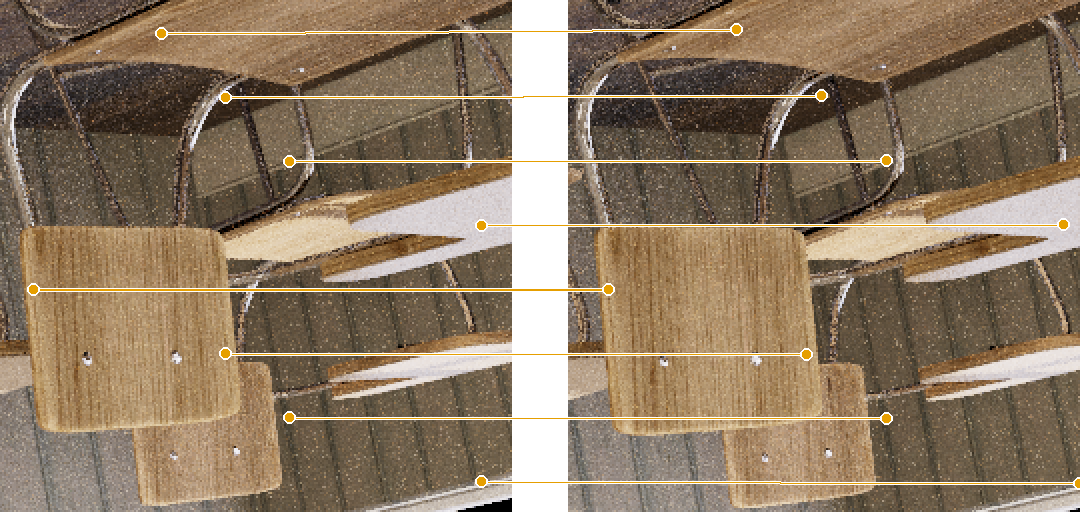
\includegraphics[width=9.7cm]{figures/fig2-pair.png}};
\node[lab] at (pair.north west) {(a) LEFT FOVEA};
\node[lab] at ($(pair.north west)+(5.1,0)$) {RIGHT FOVEA};
\node[anchor=north west, inner sep=0] (depth) at (11.05,0) {
\includegraphics[width=4.6cm]{figures/fig2-depth.png}};
\node[lab] at (depth.north west) {(b) METRIC DEPTH, LEFT GRID};
\node[anchor=north, inner sep=0] (bar) at ($(depth.south)+(0,-0.08)$) {\depthbar{4.4}};
\draw[flow] ($(pair.east)+(0.08,0)$) -- node[note, above, text width=1.2cm]{oracle\\pairs} node[note, below,
  text width=1.25cm]{triangu-\\lation} ($(depth.west)+(-0.08,0)$);
\node[anchor=north west, inner sep=0] (patch) at (0,-6.05) {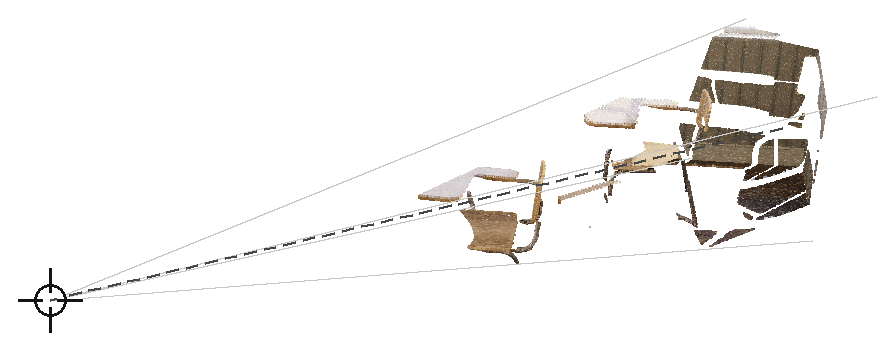
\includegraphics[width=6.3cm]{figures/fig2-patch3d.png}};
\node[lab] at (patch.north west) {(c) LOCAL METRIC PATCH IN \Hz{}};
\node[anchor=north west, inner sep=0] (cov) at (8.15,-5.75) {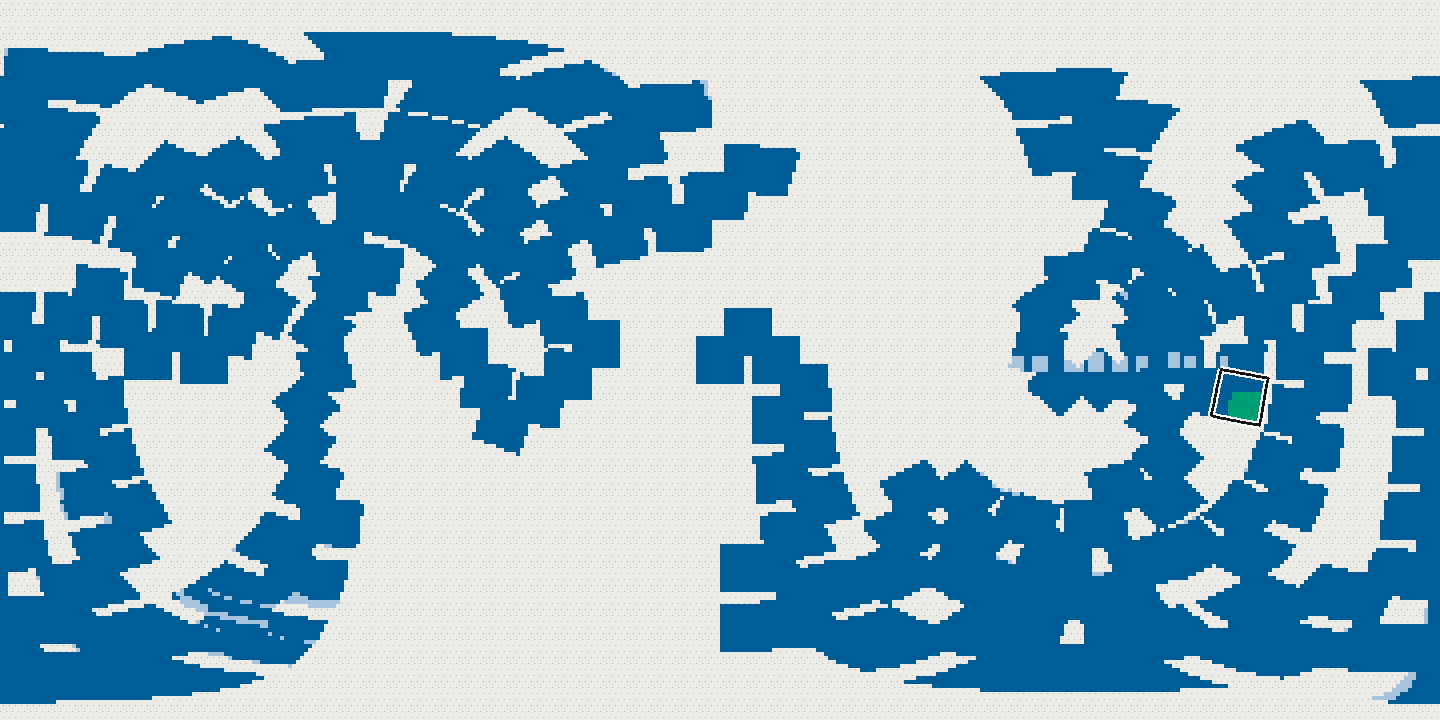
\includegraphics[width=7.55cm]{figures/fig2-coverage.png}};
\node[lab] at (cov.north west) {(d) COVERAGE MEMORY $S$ AFTER \#179};
\draw[flow] ($(pair.south west)+(2.4,-0.08)$) -- node[note, right, align=left]{same points, in \Hz{}} ($(patch.north west)+(2.4,0.42)$);
\draw[flow] ($(patch.east)+(0.1,0)$) -- node[note, above, text width=1.45cm]{fuse into $M$} node[note, below, text width=1.45cm]{update $S$} ($(patch.east)+(1.7,0)$);
\end{tikzpicture}
\caption{\textbf{One fixation (\#179, gaze yaw $130.0\degr$, pitch $-9.3\degr$).}
(a) The binocular foveal pair ($256\times256$ px each; 64-spp render, display RGB), with eight corresponding pixels,
one per epipolar row. Corresponding points share a row, and their horizontal offset is the disparity. These are
\truth{ORACLE} correspondences, shown by reprojecting the triangulated points (\truth{DERIVED}).
(b) Range from the left eye on the left foveal grid (\truth{DERIVED}); 0.5--5.5\,m scale.
(c) The fixation's 60{,}778 metric points in \Hz{}, seen obliquely, with the head (crosshair), the gaze ray (dashed)
and the 12\degr{} core (grey lines) (\truth{DERIVED}).
(d) The cyclopean coverage after this fixation (\truth{CONTROLLER-TIME}): \textsc{depth} dark blue, \textsc{seen}
light blue, \textsc{unseen} stippled grey. Green marks the cells this fixation added; the black outline is its
12\degr{} footprint. The fusion matched 36{,}481 points to existing surfels and created 24{,}297 new ones; the map grew
to 8{,}836{,}458 surfels (MEASURED).}
\label{fig:fixation}
\end{figure}

% ================================================================ 6
\section{Persistent 3-D reconstruction}\label{sec:map}

\paragraph{One global map.} All geometry from all fixations goes into a single surfel map $M$ in \Hz{}. It follows the
project's accepted 12-mm association and fusion rule, re-implemented with a vectorized spatial hash and applied to all
geometry together, with no per-object partition.

\paragraph{Association.} For each new patch, association is done against a \emph{snapshot} of the map as it was before
the patch. Each point is matched to the nearest existing surfel strictly within 12\,mm. The search covers the 27
neighbouring 12-mm hash cells and is exact; ties go to the earliest surfel. Points of the same patch never match each
other.

\paragraph{Fusion.} All points of the patch that matched the same surfel are averaged into one contribution
$\bar{\mathbf{x}}$, and that contribution is blended into the surfel with its support count $s$ as weight:
\begin{equation}
  \mathbf{x}' = \frac{s\,\mathbf{x} + \bar{\mathbf{x}}}{s + 1}, \qquad s \leftarrow s + 1 .
  \label{eq:fusion}
\end{equation}
RGB is blended in the same way; it serves display only and never enters association, coverage or gaze. Every
unmatched point becomes a new surfel, with support 1 and a record of the fixation that created it. Unmatched points
are not de-duplicated against each other within a patch. A patch identifier can be fused only once.

\paragraph{Attributes.} Each surfel stores its position, blended RGB, support count and first fixation. It also
stores the oracle Object Index of its creating point, which is used only for a segmentation-coloured visualization.
Support counts and first-fixation provenance make it possible to trace when and how often each part of the scene was
measured.

\paragraph{Storage, honestly.} The map is deliberately unoptimized. MEASURED for the official run: the final map holds
16{,}517{,}811 surfels and its archive is about 1\,GB (991\,MB); the complete run directory, including every
fixation's point patch, is 2.2\,GB. Fusion is the largest host-side cost, 257.8\,s of the 733\,s wall time. It grows
with the map, from a mean of 0.23\,s per fixation over the first 100 fixations to 0.79\,s over the last 92, with a
maximum of 2.95\,s. Compact representations are an obvious playground experiment (Section~\ref{sec:extension}).

% ================================================================ 7
\section{Cyclopean coverage memory}\label{sec:coverage}

The controller's memory of \emph{where it has looked} is separate from the map. It is a $180\times360$ grid of 1\degr{}
cells on the cyclopean sphere, each in one of three states:
\begin{itemize}
  \item \textsc{unseen}: never inside a fixation's footprint;
  \item \textsc{seen}: inside at least one footprint, i.e.\ looked at;
  \item \textsc{depth}: looked at, \emph{and} a reconstructed metric point lies in that direction from the \Hz{}
        origin.
\end{itemize}
A fixation's footprint consists of the cells whose centre falls inside its nominal 12\degr{} square core, measured in
the tangent frame ($|u|,|v| \le \tan 6\degr$). States only increase: a cell can go from \textsc{unseen} to
\textsc{seen} to \textsc{depth}, never back. We write
\[
  S_{\mathrm{seen}} = \{\,c : \mathrm{state}(c) \ge \textsc{seen}\,\}, \qquad
  S_{\mathrm{depth}} = \{\,c : \mathrm{state}(c) = \textsc{depth}\,\}.
\]

\paragraph{Solid angle, not cell counts.} An equirectangular grid has the same number of cells in every row, but a row
near a pole covers far less of the sphere than a row at the equator. Counting cells would therefore overweight the
poles. Every fraction is computed with the exact solid angle of each cell. For a row bounded by latitudes
$\phi_{\mathrm{top}}$ and $\phi_{\mathrm{bottom}}$ and a longitude width $\Delta\lambda$,
\begin{equation}
  \Delta\Omega = \Delta\lambda\,\bigl(\sin\phi_{\mathrm{top}} - \sin\phi_{\mathrm{bottom}}\bigr),
  \label{eq:solidangle}
\end{equation}
and the weights of all cells sum to exactly $4\pi$. The \textsc{seen} and \textsc{depth} fractions reported below are
fractions of $4\pi$.

\paragraph{Observation, measurement and geometry.} The three terms are kept apart. \textsc{seen} records
\emph{observation}: the fovea was pointed there. \textsc{depth} records \emph{measurement}: the fixation produced
metric points in that direction. The map $M$ holds the \emph{reconstructed geometry} itself. Coverage is updated from
the current fixation's points; it never queries the map. A \textsc{seen} cell without depth is a direction that was
looked at but returned no measurement, for instance a window with nothing behind it.

\paragraph{Seams and poles.} Longitude wraps around, so column indices are taken modulo 360. When unexplored regions
are labelled (Section~\ref{sec:policy}), the polar rows are linked across the pole. The footprint is computed from
direction dot products and has no seam at all.

Figure~\ref{fig:coverage} shows the coverage memory at four stages of the run.

\begin{figure}[t]
\centering
\begin{subfigure}[t]{0.49\linewidth}\centering
  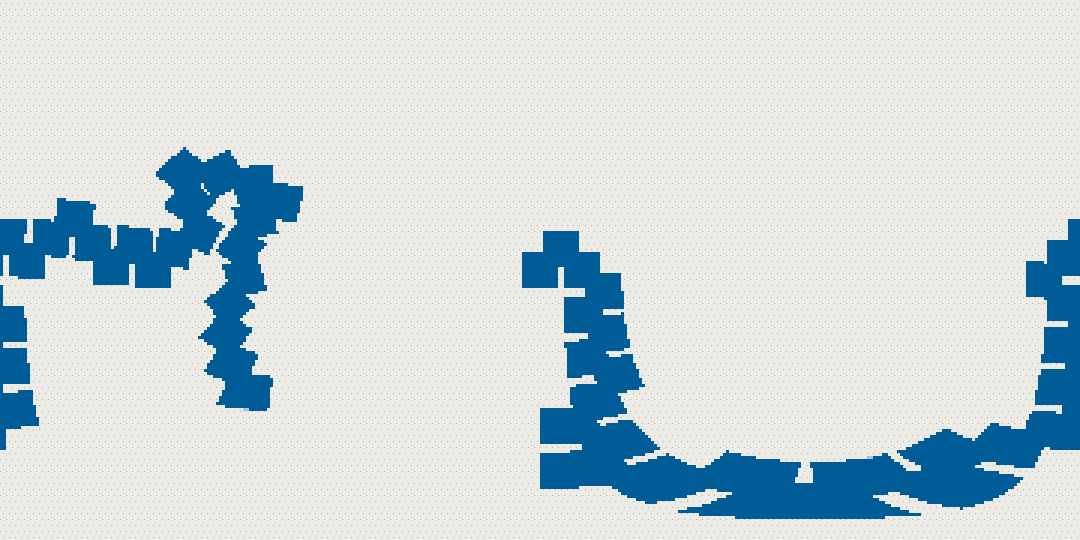
\includegraphics[width=\linewidth]{figures/fig3-coverage-0050.png}
  \caption{after \#50: \textsc{seen} \pct{14.74}, \textsc{depth} \pct{14.73}}
\end{subfigure}\hfill
\begin{subfigure}[t]{0.49\linewidth}\centering
  
\includegraphics[width=\linewidth]{figures/fig3-coverage-0200.png}
  \caption{after \#200: \textsc{seen} \pct{56.06}, \textsc{depth} \pct{55.55}}
\end{subfigure}\\[4pt]
\begin{subfigure}[t]{0.49\linewidth}\centering
  
\includegraphics[width=\linewidth]{figures/fig3-coverage-0450.png}
  \caption{after \#450: \textsc{seen} \pct{96.74}, \textsc{depth} \pct{95.96}}
\end{subfigure}\hfill
\begin{subfigure}[t]{0.49\linewidth}\centering
  
\includegraphics[width=\linewidth]{figures/fig3-coverage-0542.png}
  \caption{final, after \#542: \textsc{seen} \pct{99.00}, \textsc{depth} \pct{98.28}}
\end{subfigure}
\vspace{2pt}
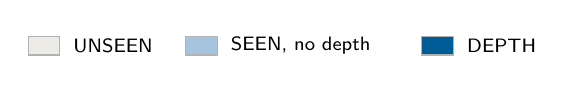
\begin{tikzpicture}[font=\sffamily\scriptsize]
  \fill[unseengrey, draw=black!30] (0,0) rectangle ++(0.4,0.24); \node[anchor=west] at (0.45,0.12) {UNSEEN};
  \fill[seenblue, draw=black!30] (2.0,0) rectangle ++(0.4,0.24); \node[anchor=west] at (2.45,0.12) {SEEN, no depth};
  \fill[depthblue, draw=black!30] (5.0,0) rectangle ++(0.4,0.24); \node[anchor=west] at (5.45,0.12) {DEPTH};
\end{tikzpicture}
\caption{\textbf{Cyclopean coverage memory at four stages} (\truth{CONTROLLER-TIME}; the state the policy actually
used). Equirectangular, yaw $-180\degr \rightarrow +180\degr$ from left to right, pitch $+90\degr$ at the top. Percentages
are fractions of $4\pi$ (MEASURED, official run). The early walk covers contiguous regions. By \#450 only scattered
small holes remain, and the final state leaves \pct{1.0} \textsc{unseen} in 184 small holes plus \pct{0.72}
\textsc{seen} without depth (mostly the windows).}
\label{fig:coverage}
\end{figure}

% ================================================================ 8
\section{Greedy saccadic exploration}\label{sec:policy}

The decision after each fixation is a pure, deterministic function of four inputs: the coverage $S$, the current
fixation's valid-geometry mask, the current gaze $g$ and the visited directions $V$. The map $M$ is \emph{not} among
them.

\paragraph{LOCAL saccades.} Eight candidates surround the current gaze in its tangent frame: E, W, N, S, NE, NW, SE and
SW. With tangent axes $x, y, z$ and $a, b \in \{-1, 0, 1\}$, a candidate direction is
$\mathbf{d} \propto z + \tan(7.2\degr)\,(a\,x + b\,y)$. Side neighbours are 7.2\degr{} away (0.6 of the core width);
diagonal neighbours are about 10.1\degr{} away. Each candidate gets two scores:
\begin{itemize}
  \item \textsc{edge\_support}: the fraction of pixels with valid reconstructed geometry in the outer quarter (64\,px)
        of the current $256\times256$ core on that side, or in the corner block for a diagonal. It asks whether the
        fovea's own measurement shows surface continuing in that direction.
  \item \textsc{unseen\_gain}: the \textsc{unseen} solid-angle fraction of the candidate's 12\degr{} footprint. It asks
        whether going there would show anything new.
\end{itemize}
A candidate is eligible if \textsc{edge\_support} $\ge 0.25$, \textsc{unseen\_gain} $\ge 0.25$ and it lies at least
2\degr{} from every visited gaze. Among eligible candidates, the one with the highest score
\begin{equation}
  \text{score} = \textsc{edge\_support} \times \textsc{unseen\_gain}
  \label{eq:score}
\end{equation}
wins; ties go to the first candidate in the fixed order above. The local rule therefore follows measured surface into
unexplored territory.

\paragraph{GLOBAL saccades.} When no neighbour is eligible, the explorer jumps:
\begin{enumerate}
  \item It labels the 4-connected components of \textsc{unseen} cells, wrapping in longitude and linking across the
        poles, and orders them by solid angle.
  \item In the largest component, it targets the \emph{deepest} cell: the cell with the largest angular distance to
        the nearest \textsc{seen} cell bordering unexplored territory, i.e.\ the middle of the hole.
  \item It skips cells within 2\degr{} of a visited gaze, falling back to the next-deepest cell and then to the next
        component.
\end{enumerate}

\paragraph{Stopping.} After each fixation, the explorer stops if \textsc{seen} $\ge \pct{99}$ of $4\pi$ (the
scientific stop), if the safety cap of 600 fixations is reached, or if no candidate remains. Otherwise it saccades.

\paragraph{What the policy does not use.} There is no object identity, no object scheduler, no semantic state and no
learned component. The oracle Object Index never reaches the policy, and neither does the 3-D map. Because the
decision is deterministic, every saved decision state can be replayed. In the official run, all 541 decisions were
re-decided identically (MEASURED, run checks).

Figure~\ref{fig:trajectory} shows the complete gaze trajectory. Panel (a) shows the local walks, each starting where a
global jump landed; panel (b) shows the 219 jumps themselves.

\begin{figure}[tbp]
\centering
\begin{tikzpicture}[font=\sffamily\scriptsize]
  \node[anchor=north west, inner sep=0] (a) at (0,0) {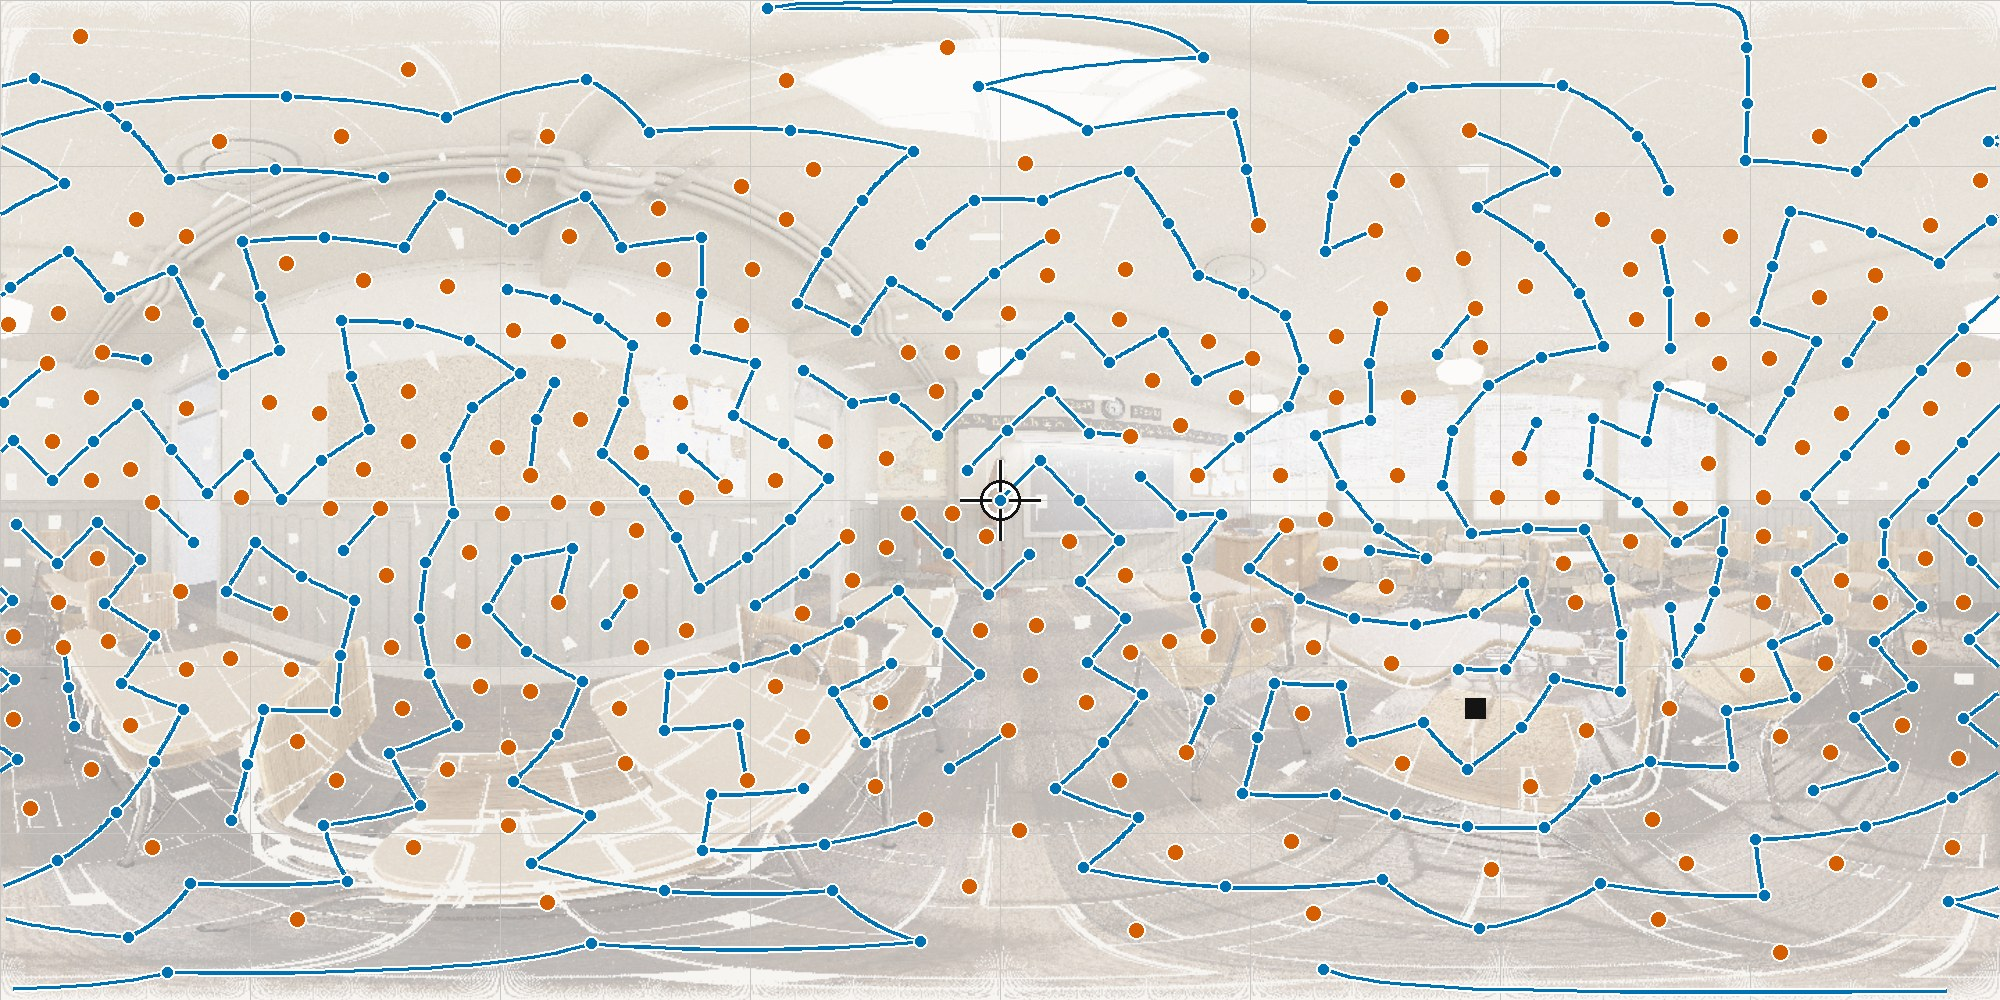
\includegraphics[width=0.92\linewidth]{figures/fig4-local.jpg}};
  \node[anchor=south west, font=\sffamily\scriptsize\bfseries, inner sep=1pt] at (a.north west)
    {(a) LOCAL WALKS: 322 local saccades; vermilion dots = landing points of global jumps};
  \draw[black!35] (a.south west) rectangle (a.north east);
  \foreach \yaw in {-180,-90,0,90,180} {\pgfmathsetmacro{\fx}{(\yaw+180)/360}
    \node[anchor=north, inner sep=1.5pt, text=black!65] at ($(a.south west)!\fx!(a.south east)$) {$\yaw\degr$};}
  \foreach \pit in {60,0,-60} {\pgfmathsetmacro{\fy}{(90-\pit)/180}
    \node[anchor=east, inner sep=1.5pt, text=black!65] at ($(a.north west)!\fy!(a.south west)$) {$\pit\degr$};}
  \node[anchor=north west, inner sep=0] (b) at ($(a.south west)+(0,-0.95)$)
    {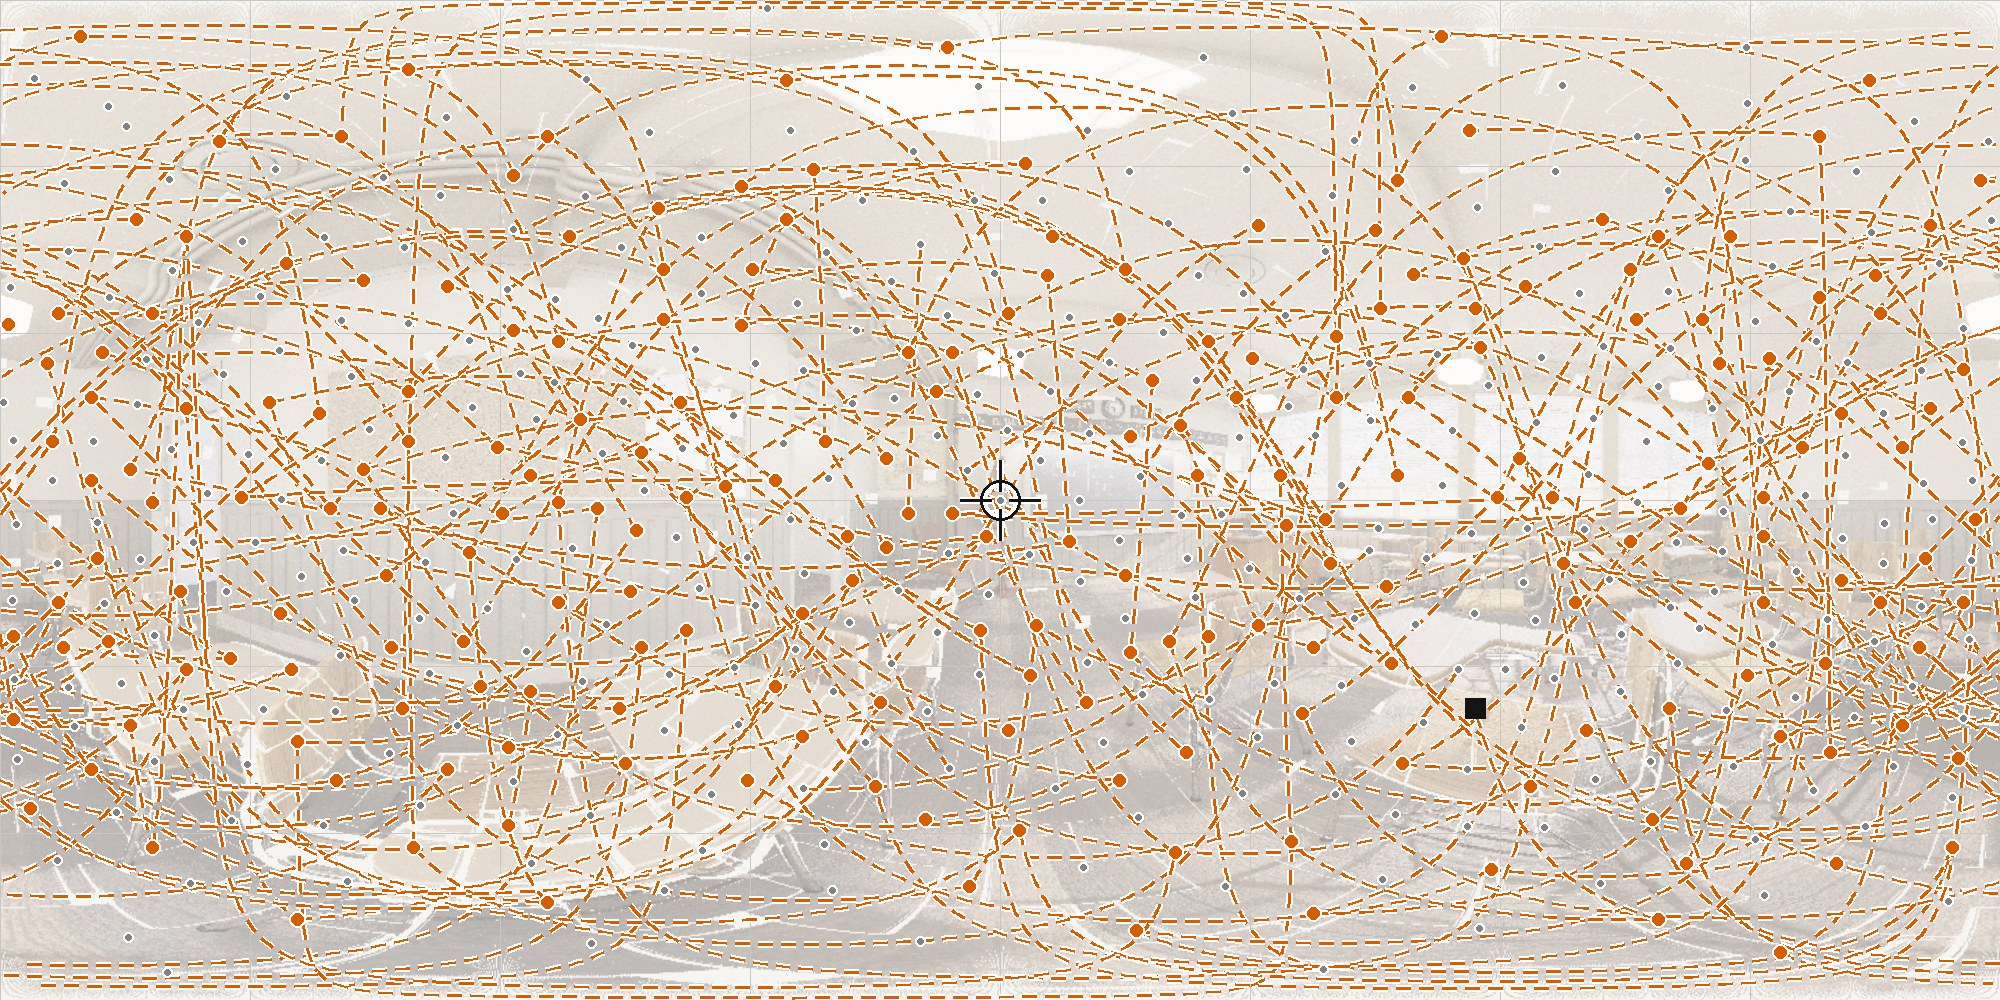
\includegraphics[width=0.92\linewidth]{figures/fig4-global.jpg}};
  \node[anchor=south west, font=\sffamily\scriptsize\bfseries, inner sep=1pt] at (b.north west)
    {(b) GLOBAL JUMPS: 219 jumps to the deepest cell of the largest unexplored region};
  \draw[black!35] (b.south west) rectangle (b.north east);
  \foreach \yaw in {-180,-90,0,90,180} {\pgfmathsetmacro{\fx}{(\yaw+180)/360}
    \node[anchor=north, inner sep=1.5pt, text=black!65] at ($(b.south west)!\fx!(b.south east)$) {$\yaw\degr$};}
  \foreach \pit in {60,0,-60} {\pgfmathsetmacro{\fy}{(90-\pit)/180}
    \node[anchor=east, inner sep=1.5pt, text=black!65] at ($(b.north west)!\fy!(b.south west)$) {$\pit\degr$};}
  % legend
  \begin{scope}[shift={($(b.south west)+(0.3,-0.75)$)}]
    \draw[white, line width=2.6pt] (0,0) -- (0.7,0); \draw[oiblue, line width=1.2pt] (0,0) -- (0.7,0);
    \node[anchor=west] at (0.75,0) {local saccade};
    \draw[oiverm, line width=1.1pt, dash pattern=on 3pt off 2pt] (3.0,0) -- (3.7,0);
    \node[anchor=west] at (3.75,0) {global jump};
    \fill[oiverm] (6.15,0) circle (0.07); \node[anchor=west] at (6.3,0) {global landing point};
    \draw[inkc, line width=0.7pt] (9.35,0) circle (0.11); \draw[inkc, line width=0.7pt] (9.15,0) -- (9.55,0)
      (9.35,-0.2) -- (9.35,0.2);
    \node[anchor=west] at (9.6,0) {start (0\degr, 0\degr)};
    \fill[inkc] (12.15,-0.08) rectangle ++(0.16,0.16); \node[anchor=west] at (12.38,0) {end, \#542};
  \end{scope}
\end{tikzpicture}
\caption{\textbf{The complete 542-fixation gaze trajectory over the 360\degr{} sphere} (\truth{CONTROLLER-TIME}; gazes
and decisions from the official run). Equirectangular, yaw left to right, pitch up. The background is the final
reconstructed RGB panorama, lightened (\truth{DERIVED}). (a) Local saccades (solid blue) form short walks that follow
measured surface into unexplored territory. (b) Global jumps (dashed vermilion) carry the gaze to the middle of the
largest remaining hole; late in the run, most of them land in small isolated holes. Grey dots in (b) are the other
fixations.}
\label{fig:trajectory}
\end{figure}

% ================================================================ 9
\section{Software architecture and reproducibility}\label{sec:software}

\paragraph{Code.} The official implementation is small: five source files plus an equivalence checker, in the
repository directory \code{tools/greedy\_foveal/} (Table~\ref{tab:software}). The canonical technical description is the
architecture document \code{docs/architecture/greedy-foveal-playground.md}.

\begin{table}[h]
\centering\small
\caption{The official implementation (\code{tools/greedy\_foveal/}).}
\label{tab:software}
\begin{tabularx}{\linewidth}{@{}l l X@{}}
\toprule
file & runs in & role \\
\midrule
\code{explorer.py} & host Python & sphere grid and coverage; one fixation's correspondence and reconstruction; the
  global map and fusion; the greedy policy \\
\code{run.py} & host Python & the active loop (\code{explore}), freeze, post-hoc \code{evaluate}, \code{checks},
  \code{visualize} \\
\code{render\_server.py} & Blender & persistent binocular observation service \\
\code{visuals.py} & host Python & overview figure; display colours for the exported point clouds \\
\code{demo.py} & host Python & offline presentation replay of the frozen run (video, poster, stills) \\
\code{check\_equivalence.py} & host Python & source, run and self-test equivalence checks against the frozen
  baseline \\
\bottomrule
\end{tabularx}
\end{table}

\paragraph{A persistent observation service.} Starting Blender and loading the scene for every fixation would dominate
the run time. The render server instead loads the Classroom once and then only moves the two eye cameras. MEASURED, a
64-spp binocular pair takes about 0.76\,s. The host and the server talk through an atomic file protocol. The host
writes a request \code{req-NNNN.json} (fixation number, yaw, pitch, output directory). The server writes the
calibration and the two images, then a \code{done-NNNN.json} marker. A failure writes \code{fail-NNNN.json} and exits
nonzero, and a \code{stop} file ends the loop. At start-up the server checks that the scene's eye pose equals the
accepted fixed head, and every fixation re-checks that the head has not moved and that the rendered gaze equals the
requested one.

\paragraph{Run stages.} A run proceeds as
\begin{center}
\sffamily explore $\rightarrow$ freeze $\rightarrow$ evaluate $\rightarrow$ checks $\rightarrow$ visualize .
\end{center}
\code{explore} runs the loop and saves, per fixation, the calibration, the point patch and the decision state. At the
end it writes the trajectory, the coverage record, the final map and two point-cloud exports, and \emph{freezes} them
by recording their SHA-256 hashes. \code{evaluate} refuses to run unless the frozen products are intact.
\code{checks} verifies invariants: the head stayed fixed; every point is finite; no fixation is repeated;
\textsc{seen} never decreased; the map reloads identically; every decision re-decides identically; and the fusion code
reproduces the accepted fusion rule bitwise on a known-answer test.

\paragraph{The truth firewall.} The evaluation reference is \emph{unavailable during control}. An audit hook records
every file the host opens during \code{explore}, and the freeze record states that none of them belongs to the
reference. Only after verifying the freeze does \code{evaluate} open the reference. MEASURED for the official run:
3{,}813 files were opened during control, none of them under the reference.

\paragraph{Dependencies.} The explorer reuses accepted project modules without copying them. By role, these are:
sensor geometry and spherical epipolar triangulation (\emph{core runtime}); the oracle correspondence, an EXR reader
and the Blender acquisition helpers (\emph{synthetic observation}); the full-sphere reference extraction and the 12-mm
coverage measure (\emph{post-hoc evaluation}); and the project's visual-language style module (\emph{presentation}).
Three data dependencies sit outside version control: the Blender scene, the accepted head-pose calibration and the
reference image (the last two hash-checked). The architecture document gives the full map.

\subsection{Official baseline and bitwise reproduction}\label{sec:equivalence}

The baseline was first run as a prototype and frozen: run, implementation and demo were each recorded by hash and
version-control tag. It was then promoted into an official, tagged code baseline (tag
\code{greedy-foveal-playground-baseline}). The promotion changed only documentation strings, and it was mechanically
checked: each promoted file is identical to its frozen version once docstrings are removed. A clean run of the official
code was then compared with the frozen run by an equivalence checker. Its rules were declared before the run:
control-path products must be \emph{bitwise} equal, and only presentation RGB may differ. GPU path tracing is not
bitwise reproducible from run to run, and RGB never enters gaze, association, coverage or stopping.

The result (MEASURED): \textbf{23 of 23 strong-equivalence checks pass}. Every one of the 542 gazes, decisions and
local-candidate scores; every per-fixation point patch and oracle label; every fusion count; all 541 decision states;
the coverage history; the final map's positions, support counts and provenance; and the post-hoc evaluation are
bitwise identical to the frozen run. The checker's own comparators were shown to fail on deliberately perturbed inputs
(a one-ULP change in a coordinate, a flipped decision, a changed constant). A 75-fixation run compared against the
full baseline fails it, as it should. For a baseline that is meant to be compared against, this is the property that
matters: any later difference is caused by the component that was changed, not by drift in the baseline.

% ================================================================ 10
\section{The Classroom proof of concept}\label{sec:classroom}

\paragraph{Setting.} The scene is the Blender Classroom, a furnished room with desks, chairs, walls, windows, a
blackboard and ceiling fixtures. Everything is static. The head is fixed at the room position given in
Section~\ref{sec:geometry}. Observations are rendered at 64 samples per pixel. Correspondence is PERFECT / ORACLE
(Section~\ref{sec:fixation}).

\paragraph{The run.} The explorer starts looking straight ahead and runs until \textsc{seen} $\ge \pct{99}$ of $4\pi$.
A safety cap of 600 fixations would have stopped it otherwise; the cap was not reached. Nothing in the run was tuned to
this scene beyond the parameters of Table~\ref{tab:params}.

\paragraph{Reference and metric.} The reconstruction is evaluated against an independent full-sphere reference: one
$720\times360$ equirectangular render (0.5\degr{} cells) from the head origin. It records, for every direction, the
first surface hit (\truth{REFERENCE / EVALUATION; NOT AVAILABLE DURING CONTROL}).
\begin{itemize}
  \item Of its 259{,}200 cells, 255{,}758 have a first hit; the other 3{,}442 look through windows into empty space.
  \item A reference cell counts as \emph{reconstructed} if some surfel of the final map lies within 12\,mm of its
        first-hit point.
  \item Coverage is reported per cell and, with exact 0.5\degr{} solid-angle weights, as a fraction of the first-hit
        reference solid angle.
\end{itemize}
The reference contains only what is visible from the head origin. Surfaces hidden behind furniture are not
reconstruction targets, and no claim is made about them.

% ================================================================ 11
\section{Results}\label{sec:results}

Table~\ref{tab:results} gives the headline numbers of the official reproduction, and Figure~\ref{fig:growth} shows how
coverage grew.

\begin{table}[h]
\centering\small
\caption{Final result of the official reproduction (MEASURED; bitwise identical to the frozen baseline in every
control-path value). Coverage percentages refer to the first-hit reference, not to all scene surfaces.}
\label{tab:results}
\begin{tabular}{@{}l r@{}}
\toprule
final fixation & 542 \\
stop reason & \textsc{seen} $\ge \pct{99}$ of $4\pi$ (cap 600 not reached) \\
\textsc{seen} (observed fraction of the sphere) & \pct{99.00} \\
\textsc{depth} (with reconstructed depth) & \pct{98.28} \\
local / global saccades & 322 / 219 \\
surfels in the final map & 16{,}517{,}811 \\
first-hit reference cells within 12\,mm & \pct{98.52} \;(251{,}966 / 255{,}758) \\
first-hit reference solid angle within 12\,mm & \textbf{\pct{98.32}} \\
\quad authored objects only (Object Index $>0$) & \pct{98.25} \\
distance to nearest surfel, covered cells & median 0.73\,mm, 90th percentile 2.24\,mm \\
wall time & 733\,s \\
\quad render / fusion / correspondence / geometry / policy & 413.5 / 257.8 / 18.2 / 12.6 / 3.3\,s \\
post-hoc evaluation & 26.3\,s \\
\bottomrule
\end{tabular}
\end{table}

\begin{figure}[t]
\centering
\begin{tikzpicture}
\begin{axis}[
  width=\linewidth, height=6.4cm, xmin=0, xmax=560, ymin=-4, ymax=104,
  xlabel={fixation number}, ylabel={fraction of the sphere ($\%$ of $4\pi$)},
  xtick={0,100,200,300,400,500}, ytick={0,20,40,60,80,100},
  axis lines=left, axis line style={black!55}, tick style={black!55},
  ymajorgrids, grid style={black!10},
  tick label style={font=\sffamily\footnotesize}, label style={font=\sffamily\small},
  legend style={at={(0.015,0.985)}, anchor=north west, draw=none, fill=white, font=\sffamily\footnotesize,
                row sep=1pt}, legend cell align=left, clip=false]
\addplot[oisky, line width=2.2pt] table[x=fixation, y=seen, col sep=comma]{figures/fig5-growth.csv};
\addlegendentry{SEEN}
\addplot[depthblue, line width=0.9pt] table[x=fixation, y=depth, col sep=comma]{figures/fig5-growth.csv};
\addlegendentry{DEPTH}
\addplot[only marks, mark=|, mark size=2.2pt, oiverm, mark options={line width=0.45pt}]
  table[x=fixation, y expr=-2, col sep=comma]{figures/fig5-global.csv};
\addlegendentry{global saccade}
\foreach \k/\s in {200/56.06, 450/96.74, 542/99.00} {
  \edef\temp{\noexpand\draw[black!45, line width=0.5pt] (axis cs:\k,0) -- (axis cs:\k,\s);}\temp
}
\node[font=\sffamily\scriptsize, align=left, anchor=west, fill=white, inner sep=1.5pt] at (axis cs:206,40)
  {\textbf{\#200}\\ SEEN 56.06\,\%\\ DEPTH 55.55\,\%};
\node[font=\sffamily\scriptsize, align=right, anchor=east, fill=white, inner sep=1.5pt] at (axis cs:444,66)
  {\textbf{\#450}\\ SEEN 96.74\,\%\\ DEPTH 95.96\,\%};
\node[font=\sffamily\scriptsize, align=right, anchor=east, fill=white, inner sep=1.5pt] at (axis cs:536,40)
  {\textbf{\#542} (stop)\\ SEEN 99.00\,\%\\ DEPTH 98.28\,\%};
\end{axis}
\end{tikzpicture}
\caption{\textbf{Growth of \textmd{\textsc{seen}} and \textmd{\textsc{depth}} with fixation number} (\truth{CONTROLLER-TIME}, MEASURED,
official run). Ticks along the bottom mark the 219 global saccades. The two curves nearly coincide because almost
every direction that was looked at also returned depth. Three phases are visible: fast local exploration (few global
jumps before \#200); a mixed phase in which global jumps become frequent (\#201--\#450); and a long tail of single
global jumps into small holes (\#451--\#542).}
\label{fig:growth}
\end{figure}

\paragraph{Three phases.} The growth curve has three distinct regimes (Table~\ref{tab:phases}).
\begin{itemize}
  \item \emph{Local exploration.} For the first 68 fixations the explorer never needs to jump: local walks alone
        cover \pct{19.6} of the sphere. Through \#200 it makes 195 local and only 4 global saccades, and
        \textsc{seen} rises almost linearly to \pct{56.06}.
  \item \emph{Mixed exploration.} Between \#201 and \#450, local walks increasingly run into explored territory, and
        global jumps make up nearly half the moves (123 of 250). \textsc{seen} reaches \pct{96.74}.
  \item \emph{Hole filling.} After \#450 all 92 moves are global, each into one small isolated hole. The mean
        \textsc{seen} gain falls to \pct{0.025} per fixation (minimum \pct{0.015}).
\end{itemize}

\begin{table}[h]
\centering\small
\caption{Exploration phases (MEASURED, official run; values at the end of each phase).}
\label{tab:phases}
\begin{tabular}{@{}l c c c c@{}}
\toprule
fixations & local & global & \textsc{seen} & \textsc{depth} \\
\midrule
1--200   & 195 & 4   & \pct{56.06} & \pct{55.55} \\
201--450 & 127 & 123 & \pct{96.74} & \pct{95.96} \\
451--542 & 0   & 92  & \pct{99.00} & \pct{98.28} \\
\bottomrule
\end{tabular}
\end{table}

\paragraph{The final reconstruction.} Figure~\ref{fig:final} compares the reconstruction with the independent reference.
Projected back onto the sphere, the final map reproduces the room's appearance (RGB), its metric layout (depth) and,
for visualization only, its object structure (oracle instance labels). The 3-D view shows the room as one coherent
metric model. Post hoc, \pct{98.32} of the first-hit reference solid angle lies within 12\,mm of the map
(\pct{98.52} of reference cells). Covered cells are typically much closer than the threshold: the median distance to
the nearest surfel is 0.73\,mm. What remains has two causes. One is the 184 small \textsc{unseen} holes, each smaller
than 0.002\,sr. The other is thin slivers along depth edges, where the reference ray from the head origin meets a
surface that the binocular measurement did not reach.

\begin{figure}[tbp]
\centering
\begin{tikzpicture}[font=\sffamily\scriptsize,
  hdr/.style={font=\sffamily\scriptsize\bfseries, anchor=south west, inner sep=1pt},
  col/.style={font=\sffamily\scriptsize, anchor=south, inner sep=1pt, text=black!70}]
\def\pw{4.88}
\foreach \f/\x/\t in {rgb/0/RGB, depth/1/{DEPTH (RANGE)}, instance/2/{INSTANCE (ORACLE, VISUALIZATION ONLY)}} {
  \node[anchor=north west, inner sep=0] (f\f) at ({\x*(\pw+0.25)},0)
    {\includegraphics[width=\pw cm]{figures/fig6-final-\f}};
  \node[col] at (f\f.north) {\t};
  \node[anchor=north west, inner sep=0] (r\f) at ({\x*(\pw+0.25)},-3.25)
    {\includegraphics[width=\pw cm]{figures/fig6-reference-\f}};
}
\node[hdr] at ($(frgb.north west)+(0,0.32)$) {(a) ACTIVE RECONSTRUCTION, projected from the final map \;
  \textmd{[DERIVED]}};
\node[hdr] at ($(rrgb.north west)+(0,0.05)$) {(b) BLENDER REFERENCE \;
  \textmd{[REFERENCE / EVALUATION --- NOT AVAILABLE DURING CONTROL]}};
\node[anchor=north, inner sep=0] at ($(rdepth.south)+(0,-0.12)$) {\depthbar{4.6}};
\node[anchor=north west, inner sep=0] (map) at (0,-6.85) {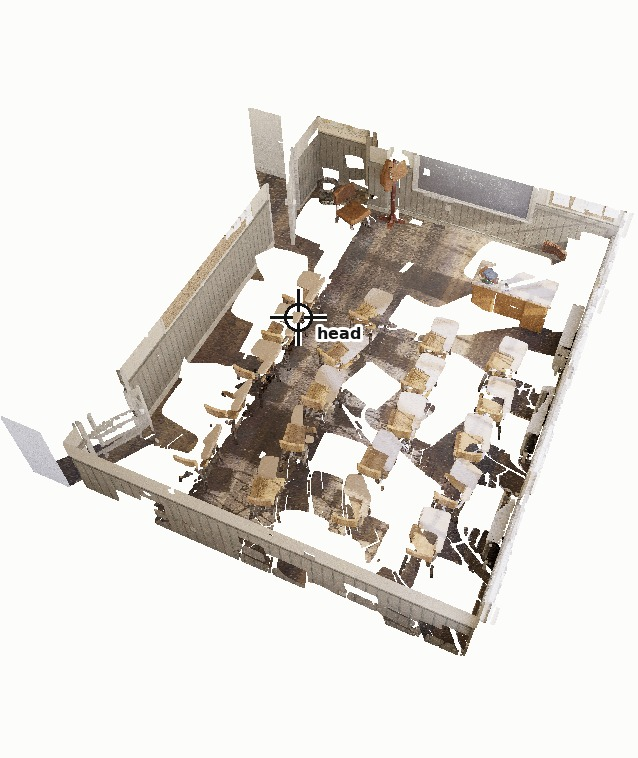
\includegraphics[height=6.1cm]{figures/fig6-map3d.jpg}};
\node[hdr] at (map.north west) {(c) FINAL 3-D MAP \textmd{[DERIVED]}};
\node[anchor=north west, inner sep=0] (ev) at (5.55,-7.3) {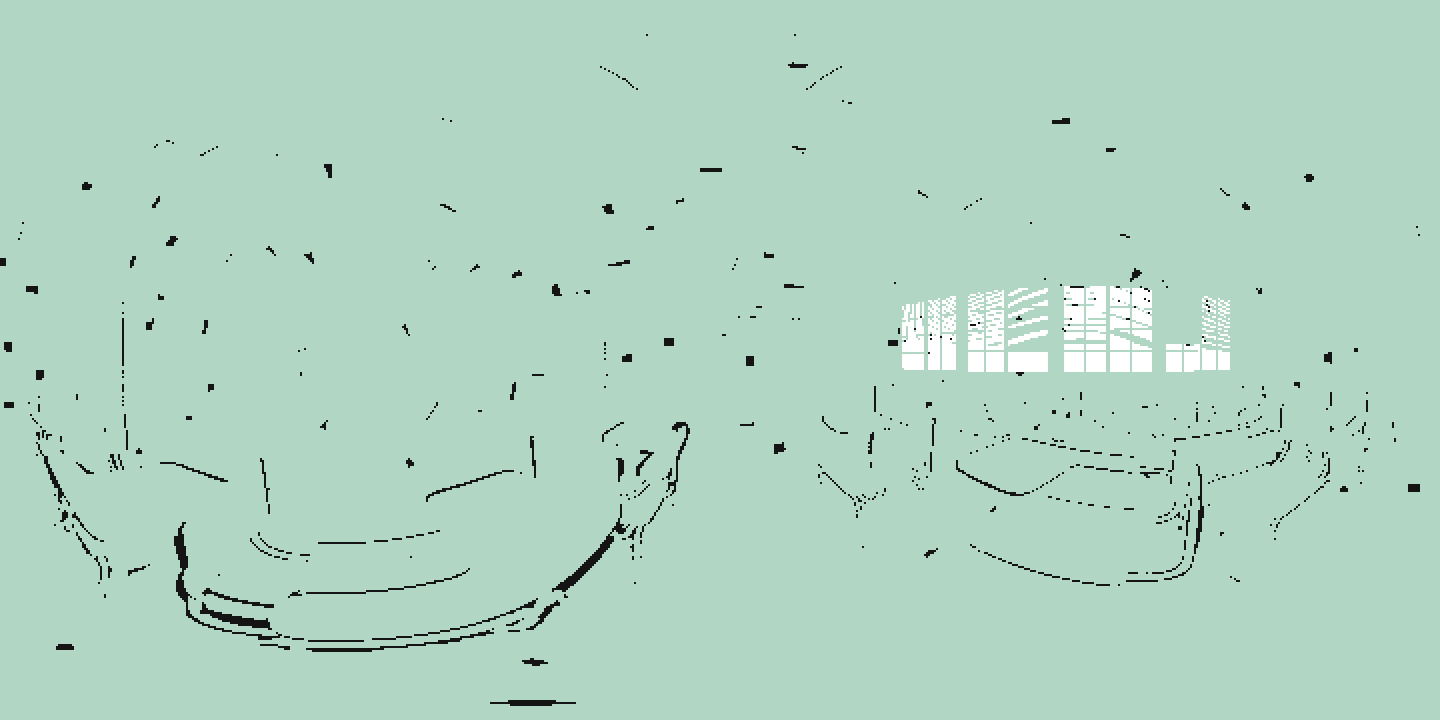
\includegraphics[width=9.5cm]{figures/fig6-evaluation.png}};
\draw[black!35] (ev.south west) rectangle (ev.north east);
\node[hdr] at (ev.north west) {(d) POST-HOC 12-MM COVERAGE \textmd{[REFERENCE / EVALUATION]}};
\begin{scope}[shift={($(ev.south west)+(0.05,-0.5)$)}]
  \fill[coveredgreen, draw=black!30] (0,0) rectangle ++(0.4,0.24); \node[anchor=west] at (0.45,0.12) {reconstructed within 12\,mm};
  \fill[inkc] (4.4,0) rectangle ++(0.4,0.24); \node[anchor=west] at (4.85,0.12) {not reconstructed};
  \draw[black!30] (7.6,0) rectangle ++(0.4,0.24); \node[anchor=west] at (8.05,0.12) {no first hit};
\end{scope}
\end{tikzpicture}
\caption{\textbf{Final reconstruction and reference.}
(a) The final map projected onto the sphere from the head origin, nearest surfel per pixel: display RGB, range, and
oracle instance labels (\truth{DERIVED}; instance colours are \truth{ORACLE / VISUALIZATION ONLY} and played no role
in the run). Stippled grey = nothing reconstructed in that direction.
(b) The independent Blender reference at 0.5\degr{} (\truth{REFERENCE / EVALUATION}, never available during control).
(c) The 16.5-million-surfel map seen from above and behind the head, with the ceiling removed for display
(\truth{DERIVED}).
(d) Post-hoc evaluation over the reference sphere: \pct{98.32} of the first-hit reference solid angle is
reconstructed within 12\,mm. The misses are small holes and thin depth-edge slivers; the windows (white) have no
first hit. Panels (a)--(c) are images from the frozen demonstration, whose control path the official reproduction
matches bitwise.}
\label{fig:final}
\end{figure}

% ================================================================ 12
\section{Discussion}\label{sec:discussion}

\paragraph{What the result establishes.} Within its controlled setting, the experiment supports five observations.
\begin{enumerate}
  \item \emph{Narrow measurements accumulate into a whole scene.} Repeated 12\degr{} binocular measurements, each
        expressed in one fixed frame and fused into one map, add up to a nearly complete metric representation of the
        first-hit 360\degr{} scene: \pct{98.32} of the reference solid angle within 12\,mm, after 542 fixations.
  \item \emph{A very simple policy is enough here.} The greedy rule has one score and two thresholds, and it uses no
        model of the scene beyond a 1\degr{} coverage grid. It stopped on its own at \pct{99} coverage, without
        stalling.
  \item \emph{Local and global gaze are complementary.} Local saccades exploit what the current fixation measured:
        they follow surfaces. Global saccades exploit what the memory knows: they go where nothing has been seen.
        Neither alone would suffice. Local walks stall at boundaries of explored territory, and pure global jumps
        would ignore the continuity that makes local walks efficient early on.
  \item \emph{Memory turns a narrow fovea into a wide-field observer.} At no moment does the system see more than
        12\degr{} in detail. Persistent memory---the map for geometry, the coverage sphere for attention---is what makes
        the accumulated percept wide.
  \item \emph{The architecture is separable.} Observation, correspondence, triangulation, fusion, coverage and policy
        meet at narrow, explicit interfaces. The truth-stripped correspondence interface is the clearest example, and
        each of these services can be replaced independently (Section~\ref{sec:extension}).
\end{enumerate}

\paragraph{What it does not establish.} The experiment says nothing about natural correspondence: matching was perfect
by construction. Nor does it show natural segmentation; the oracle labels only colour figures. It shows no optimal or
even efficient gaze selection, no perception with a moving head, no dynamic scenes, and no generalization beyond one
synthetic room. The reconstruction target is the first-hit scene seen from one point, so hidden surfaces are outside
it.

\paragraph{The map is not in the control loop.} The most important architectural observation is what the policy does
\emph{not} read. Gaze is driven by a coverage record (\emph{was this direction looked at?}) and by the current
fixation's valid-geometry mask (\emph{does measured surface continue this way?}). The accumulated 3-D map---the system's
best knowledge of the scene---is never consulted. This kept the baseline minimal, and the result shows that such a
loop can already reconstruct the first-hit scene almost completely. It also frames a sharp next question: what changes
when attention is driven by the reconstructed 3-D map? Map-driven frontiers could target depth discontinuities,
low-support regions or surfaces seen only at grazing angles. Whether that reduces the fixation count, improves the
geometry, or both, is exactly the kind of question the playground is built to answer.

\paragraph{The late global tail.} After \#450, the explorer spends 92 fixations clearing small holes one at a time,
each jump gaining on average \pct{0.025} of the sphere. Each hole is the size of a fraction of the fovea, so most of
each fixation re-measures known territory. This is not a defect to explain away. It is useful evidence about the
simple policy. A global rule that picks the \emph{largest} hole regardless of distance spends many long saccades on
small gains. Ordering the remaining holes into a short tour, or covering several holes per fixation, are obvious
alternatives---and they are measurable against this baseline.

\paragraph{On the oracle assumption.} PERFECT correspondence removes matching errors and missed matches. This report
does not estimate how natural stereo would change the measured coverage or precision. The design does guarantee,
though, that the comparison can be made cleanly: a natural matcher plugs into the same interface, and everything
downstream stays fixed.

% ================================================================ 13
\section{The playground}\label{sec:extension}

The accepted baseline is intentionally not optimal. Its value is that it is complete, simple, explicit and exactly
reproducible, so that the effect of changing one component can be measured. The research method it supports is:
\begin{center}
\sffamily change ONE component $\;\rightarrow\;$ compare against the official baseline $\;\rightarrow\;$ measure the
causal effect
\end{center}
Table~\ref{tab:extension} lists the replaceable components and Figure~\ref{fig:extension} shows where they sit in the
loop.

\begin{table}[h]
\centering\small
\caption{Playground extension points. Each row can be replaced independently; the architecture document gives each
component's interface.}
\label{tab:extension}
\begin{tabularx}{\linewidth}{@{}l X X@{}}
\toprule
component & current baseline & replaceable by (examples) \\
\midrule
renderer & Blender Cycles, persistent server, 64 spp & other scenes; other sample counts; a fast rasterizer; real cameras \\
stereo matcher & PERFECT / ORACLE correspondence & natural stereo (block matching, learned matchers) \\
local measurement & spherical epipolar triangulation & per-point uncertainty; surface normals; variable fovea \\
map representation & flat float64 surfel arrays & compact surfels; voxel / TSDF / octree maps \\
fusion & 12-mm snapshot association, support-weighted mean & confidence weighting; outlier rejection; de-duplication \\
coverage representation & 1\degr{} \textsc{unseen}/\textsc{seen}/\textsc{depth} sphere & finer or equal-area grids;
  graded confidence \\
local gaze policy & 8 neighbours, edge support $\times$ unseen gain & map-driven 3-D frontiers; information gain \\
global gaze policy & deepest cell of the largest unexplored region & nearest-hole or tour ordering of holes \\
stopping rule & \textsc{seen} $\ge \pct{99}$, cap, no candidate & depth- or quality-based stop; time budget \\
segmentation / semantics & none in control (oracle labels for figures) & natural segmentation; object-aware attention \\
head motion & none: fixed head & head pose as an action; better-conditioned stereo \\
visualization & overview figure, offline demo replay & interactive viewer; web presentation \\
\bottomrule
\end{tabularx}
\end{table}

\begin{figure}[t]
\centering
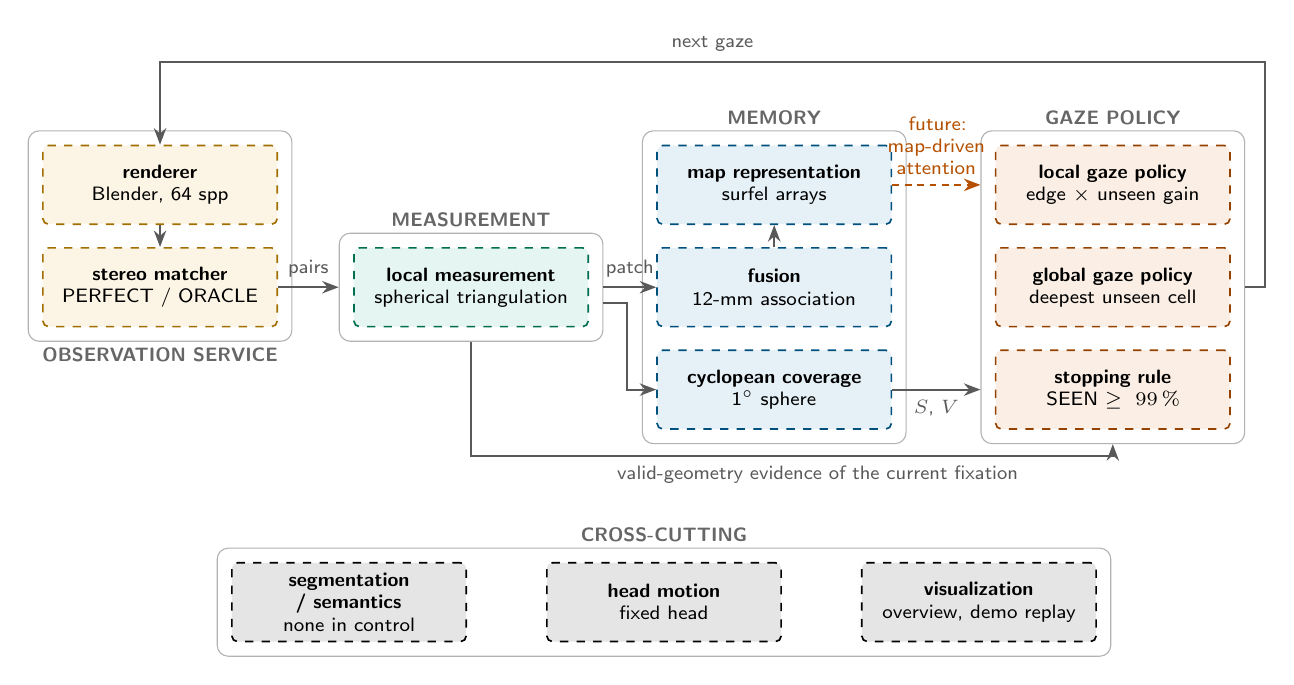
\begin{tikzpicture}[font=\sffamily\scriptsize, >={Stealth[length=2.1mm]},
  comp/.style={draw=#1!70!black, fill=#1!10, rounded corners=2pt, line width=0.6pt, dashed, align=center,
               text width=2.8cm, minimum height=1.0cm, inner sep=2.5pt},
  group/.style={draw=black!30, rounded corners=4pt, inner sep=5pt},
  grp/.style={font=\sffamily\scriptsize\bfseries, text=black!60, anchor=south, inner sep=2pt},
  note/.style={font=\sffamily\scriptsize, text=black!65, align=center},
  flow/.style={->, line width=0.75pt, black!65}]
\node[comp=oiorange] (ren) at (0,0.95) {\textbf{renderer}\\ Blender, 64 spp};
\node[comp=oiorange] (mat) at (0,-0.35) {\textbf{stereo matcher}\\ PERFECT / ORACLE};
\node[comp=oigreen]  (meas) at (3.95,-0.35) {\textbf{local measurement}\\ spherical triangulation};
\node[comp=oiblue]   (map) at (7.8,0.95) {\textbf{map representation}\\ surfel arrays};
\node[comp=oiblue]   (fus) at (7.8,-0.35) {\textbf{fusion}\\ 12-mm association};
\node[comp=oiblue]   (cov) at (7.8,-1.65) {\textbf{cyclopean coverage}\\ 1\degr{} sphere};
\node[comp=oiverm]   (loc) at (12.1,0.95) {\textbf{local gaze policy}\\ edge $\times$ unseen gain};
\node[comp=oiverm]   (glo) at (12.1,-0.35) {\textbf{global gaze policy}\\ deepest unseen cell};
\node[comp=oiverm]   (stp) at (12.1,-1.65) {\textbf{stopping rule}\\ SEEN $\ge \pct{99}$};
\begin{scope}[on background layer]
  \node[group, fit=(ren)(mat)] (gobs) {};
  \node[group, fit=(meas)] (gmeas) {};
  \node[group, fit=(map)(fus)(cov)] (gmem) {};
  \node[group, fit=(loc)(glo)(stp)] (gpol) {};
\end{scope}
\node[grp, anchor=north] at (gobs.south) {OBSERVATION SERVICE};
\node[grp] at (gmeas.north) {MEASUREMENT};
\node[grp] at (gmem.north) {MEMORY};
\node[grp] at (gpol.north) {GAZE POLICY};
% baseline data flow
\draw[flow] (ren.south) -- (mat.north);
\draw[flow] (mat.east) -- node[note, above]{pairs} (gmeas.west |- mat.east);
\draw[flow] (gmeas.east |- fus.west) -- node[note, above]{patch} (fus.west);
\draw[flow] ($(gmeas.east)+(0,-0.2)$) -- ++(0.3,0) |- (cov.west);
\draw[flow] (fus.north) -- (map.south);
\draw[flow] (cov.east) -- node[note, below]{$S$, $V$} (gpol.west |- cov.east);
\draw[flow] (gmeas.south) -- ++(0,-1.45) -| node[note, pos=0.27, below]{valid-geometry evidence of the current fixation}
  (gpol.south);
\draw[flow] (gpol.east) -- ++(0.25,0) |- ($(ren.north)+(0,1.05)$) node[note, pos=0.75, above]{next gaze} -- (ren.north);
% the absent edge
\draw[->, line width=0.85pt, dash pattern=on 2.5pt off 2pt, oiverm!85!black] (map.east) -- node[above, note,
  text=oiverm!85!black, text width=1.4cm]{future: map-driven attention} (gpol.west |- map.east);
% cross-cutting
\node[comp=black] (seg) at (2.4,-4.35) {\textbf{segmentation / semantics}\\ none in control};
\node[comp=black] (head) at (6.4,-4.35) {\textbf{head motion}\\ fixed head};
\node[comp=black] (vis) at (10.4,-4.35) {\textbf{visualization}\\ overview, demo replay};
\begin{scope}[on background layer]\node[group, fit=(seg)(head)(vis)] (gx) {};\end{scope}
\node[grp] at (gx.north) {CROSS-CUTTING};
\end{tikzpicture}
\caption{\textbf{Playground extension map.} Every dashed box is a replaceable component, coloured by role:
observation (orange), measurement (green), memory (blue), gaze policy (vermilion), cross-cutting (grey). Solid arrows
are the data flow of the baseline. The dashed vermilion arrow from the map to the policy is \emph{not} part of the
baseline: map-driven attention is a future experiment, and in the baseline the policy reads coverage, visited
directions and the current fixation's evidence only.}
\label{fig:extension}
\end{figure}

\paragraph{Possible directions.} Without selecting the next experiment, the playground invites several:
\begin{itemize}
  \item \emph{natural stereo}, through the truth-stripped correspondence interface;
  \item \emph{map-driven frontier exploration}, closing the loop from $M$ to the policy;
  \item \emph{smarter global saccade ordering} for the hole-filling tail;
  \item \emph{compact map representations} that keep fusion semantics while cutting memory and time;
  \item \emph{natural segmentation and semantics}, to give attention an object-level vocabulary without oracles;
  \item a \emph{moving head}, so that stereo can be re-centred where it is poorly conditioned;
  \item \emph{new scenes}, to test whether the baseline's behaviour transfers;
  \item \emph{actual foveated, variable-resolution sensing}, replacing the uniform render with a retina-like sampling.
\end{itemize}
Each of these changes one row of Table~\ref{tab:extension}. Each can be judged against the same frozen numbers:
fixations to \pct{99} \textsc{seen}, the growth curve, first-hit coverage, map size and time.

% ================================================================ 14
\section{Limitations}\label{sec:limitations}

The baseline is defined by its limitations as much as by its results. Stating them precisely is what makes it usable
as a reference.
\begin{itemize}
  \item \textbf{Fixed head.} Only the eyes move. The head position is a parameter, and poorly conditioned
        near-baseline gazes cannot be avoided by moving it.
  \item \textbf{Static synthetic scene.} One Blender room, with no motion, no lighting change and no sensor noise
        model beyond Monte Carlo render noise.
  \item \textbf{PERFECT / ORACLE correspondence.} Matches come from the renderer's geometry; no natural stereo is
        involved.
  \item \textbf{Oracle labels only where declared.} Object Index is used by the correspondence oracle and for
        visualization. It never drives gaze, fusion or stopping.
  \item \textbf{64-spp synthetic observation.} RGB is noisy and not bitwise reproducible. Under PERFECT correspondence
        it affects display only.
  \item \textbf{First-hit evaluation.} The target is what is visible from the head origin. Hidden and occluded
        surfaces are outside the target set.
  \item \textbf{An unsophisticated greedy trajectory}, with a diagonal bias in local walks, triangular holes and a long
        hole-filling tail.
  \item \textbf{The map is not used for control.} The policy never consults the reconstruction.
  \item \textbf{Storage is not optimized}: about 1\,GB for the final map and 2.2\,GB per run.
  \item \textbf{One demonstrated scene.} Nothing here shows transfer to other environments.
\end{itemize}

% ================================================================ 15
\section{Conclusion}\label{sec:conclusion}

We set out to ask whether a narrow, spatially selective binocular observer could build a persistent 3-D
representation of its surroundings by choosing where to look. In a controlled synthetic setting it can. A loop of
fixation, local metric reconstruction, persistent memory and a simple greedy saccade rule observed \pct{99} of the
sphere in 542 fixations, and reconstructed \pct{98.32} of the first-hit reference solid angle within 12\,mm. The
implementation reproduces this result bitwise.

The important result is not that a greedy policy is optimal; it plainly is not. It is that a small, explicit
active-foveal loop is enough to produce a complete and reproducible computational baseline. That changes the question.
It is no longer \emph{whether} active foveal reconstruction can work, but \emph{which component to replace next}, and
by how much the change helps.

\bibliographystyle{plainnat}
\bibliography{references}

% ================================================================ appendix
\appendix
\section{Reproduction and provenance}\label{app:provenance}

\paragraph{Repository and tags.}
\begin{itemize}
  \item repository: \url{https://github.com/visgraf/f3d-vision}
  \item official baseline: annotated tag \code{greedy-foveal-playground-baseline} (commit \code{203a70c})
  \item frozen prototype implementation: tag \code{greedy-foveal-explorer-v0-impl}
  \item frozen demonstration: tag \code{greedy-foveal-explorer-v0-demo}
\end{itemize}

\paragraph{Canonical documents.}
\begin{itemize}
  \item architecture (the canonical technical description):\\ \code{docs/architecture/greedy-foveal-playground.md}
  \item official reproduction and equivalence evidence:\\
        \code{docs/engineering/greedy-foveal-playground-baseline-report.md}
  \item proof-of-concept closure, with the hashes of the frozen run and demo:\\
        \code{docs/prototype/greedy-foveal-explorer-v0-closure.md}
\end{itemize}

\paragraph{Commands.} From the repository root (Blender 5.2.1 with an OPTIX GPU; about 12 minutes on an RTX 4090):
{\footnotesize
\begin{verbatim}
.venv/bin/python tools/greedy_foveal/run.py explore  --run RUN --max-fix 600 --spp 64
.venv/bin/python tools/greedy_foveal/run.py evaluate --run RUN
.venv/bin/python tools/greedy_foveal/run.py checks   --run RUN
.venv/bin/python tools/greedy_foveal/check_equivalence.py run --run RUN \
    --baseline previews/greedy-foveal-explorer-v0-grow600 --known-answer
\end{verbatim}}

\paragraph{Measured source of this report.} All MEASURED values come from the official reproduction run
(\nolinkurl{previews/greedy-foveal-official-baseline/}, freeze record SHA-256 \code{6bc9b190\ldots}). It was made from
commit \code{b77b1d9} and is bitwise equivalent to the frozen run in every control-path product. The figures were
produced by \nolinkurl{docs/technical-report/make_figures.py} from that run and from the frozen demonstration's images.
No scene was rendered for this report. \nolinkurl{figures/figure-sources.json} records the hash of every input and output.

\end{document}
